\documentclass[11pt,a4paper]{article}

\usepackage{fontspec}
\usepackage[margin=24mm]{geometry}
\usepackage{amsmath,amssymb,mathtools}
\usepackage{booktabs,longtable,array,tabularx}
\usepackage{caption}
\usepackage{graphicx}
\usepackage{xcolor}
\usepackage{hyperref}
\usepackage{enumitem}

\defaultfontfeatures{Ligatures=TeX,Scale=MatchLowercase}
\IfFontExistsTF{Noto Sans CJK KR}{
  \setmainfont{Noto Sans CJK KR}[
    ItalicFeatures={FakeSlant=0.18},
    BoldItalicFeatures={FakeSlant=0.18}
  ]
  \setsansfont{Noto Sans CJK KR}[
    ItalicFeatures={FakeSlant=0.18},
    BoldItalicFeatures={FakeSlant=0.18}
  ]
}{
  \IfFontExistsTF{Apple SD Gothic Neo}{
    \setmainfont{Apple SD Gothic Neo}[
      ItalicFeatures={FakeSlant=0.18},
      BoldItalicFeatures={FakeSlant=0.18}
    ]
    \setsansfont{Apple SD Gothic Neo}[
      ItalicFeatures={FakeSlant=0.18},
      BoldItalicFeatures={FakeSlant=0.18}
    ]
  }{
    \setmainfont{NanumGothic}[
      ItalicFeatures={FakeSlant=0.18},
      BoldItalicFeatures={FakeSlant=0.18}
    ]
    \setsansfont{NanumGothic}[
      ItalicFeatures={FakeSlant=0.18},
      BoldItalicFeatures={FakeSlant=0.18}
    ]
  }
}
\IfFontExistsTF{DejaVu Sans Mono}{
  \setmonofont{DejaVu Sans Mono}
}{
  \IfFontExistsTF{Menlo}{
    \setmonofont{Menlo}
  }{
    \setmonofont{Liberation Mono}
  }
}
\XeTeXlinebreaklocale "ko"
\XeTeXlinebreakskip = 0pt plus 1pt

\hypersetup{
  colorlinks=true,
  linkcolor=blue!50!black,
  urlcolor=blue!50!black,
  citecolor=blue!50!black,
  pdftitle={MuJoCo 유체력 모델과 UUV 시뮬레이터 물리 파라미터 정리},
  pdfauthor={OpenAI Codex}
}

\setlength{\parskip}{0.6em}
\setlength{\parindent}{0pt}
\setlength{\emergencystretch}{3em}
\renewcommand{\arraystretch}{1.25}
\newcolumntype{Y}{>{\raggedright\arraybackslash}X}
\newcommand{\code}[1]{\nolinkurl{#1}}
\captionsetup{
  font=small,
  labelfont=bf,
  justification=raggedright,
  singlelinecheck=false,
  skip=6pt
}

\title{MuJoCo 유체력 모델과\\UUV 시뮬레이터 물리 파라미터 정리}
\author{}
\date{2026-04-03}

\begin{document}
\maketitle

\section{문서 목적}

이 문서는 MuJoCo 공식 문서의 \textbf{Fluid forces} 절을 기준으로, 현재 UUV 시뮬레이터에서 사용되는 물리 모델을 한국어로 정확하게 정리한 문서이다. 목적은 세 가지다.

\begin{enumerate}[leftmargin=2em]
  \item MuJoCo가 기본으로 제공하는 유체력 모델이 무엇인지 설명한다.
  \item 현재 프로젝트가 MuJoCo built-in fluid model을 그대로 쓰는지, 아니면 custom hydrodynamics를 얹고 있는지 명확히 구분한다.
  \item 실제 조정 가능한 물리 파라미터가 어떤 파일에 있고 어떤 의미를 가지는지 체계적으로 정리한다.
\end{enumerate}

핵심 결론부터 먼저 말하면 다음과 같다.

\begin{itemize}[leftmargin=2em]
  \item MuJoCo는 \textbf{inertia-based} 유체력 모델과 \textbf{ellipsoid-based} 유체력 모델을 제공한다.
  \item 이 프로젝트는 MuJoCo를 강체 적분기와 접촉/조인트 해석기로 사용하지만, 수중력의 대부분은 \textbf{Python에서 직접 계산해서 \texttt{xfrc\_applied}로 주입}한다.
  \item 따라서 현재 프로젝트는 \textbf{MuJoCo built-in passive fluid model만으로 동작하는 구조가 아니라}, MuJoCo 위에 \textbf{custom 6-DOF underwater hydrodynamics layer}를 얹은 구조다.
\end{itemize}

\section{최근 구조 변경 사항 (2026-04)}

2026년 4월 기준으로 active runtime 경로와 설치 스크립트 구조를 다시 정리했다. 이 절의 내용이 현재 코드 상태를 가장 직접적으로 반영한다.

\subsection{Active runtime 경로는 두 개만 유지}

현재 launcher와 profile은 아래 두 경로만 active로 유지한다.

\begin{center}
\small
\begin{tabularx}{\linewidth}{>{\raggedright\arraybackslash}p{0.20\linewidth}>{\raggedright\arraybackslash}p{0.24\linewidth}Y}
\toprule
구분 & active 이름 & 의미 \\
\midrule
scene & \code{tank\_custom\_scene.xml} & Python에서 계산한 custom 6-DOF hydrodynamics를 쓰는 기본 경로 \\
scene & \code{tank\_ellipsoid\_scene.xml} & MuJoCo built-in ellipsoid fluid를 쓰는 비교/실험 경로 \\
profile & \code{custom} & custom hydrodynamics용 기본 프로파일 \\
profile & \code{ellipsoid} & built-in ellipsoid 모드용 기본 프로파일 \\
\bottomrule
\end{tabularx}
\end{center}

즉 이전의 \code{sim\_simple}, \code{sim\_real}, \code{sim\_stable\_real}, \code{competition\_scene.xml} 같은 이름은 더 이상 active entrypoint가 아니다. 이전 실험 파일과 로그는 \code{uuv\_mujoco/v2.2/delete/} 로 옮겨 두었고, 확인 후 최종 삭제할 수 있게 분리했다.

\subsection{실행 스크립트 이름도 단순화}

실행 경로는 아래 두 스크립트 기준으로 정리했다.

\begin{itemize}[leftmargin=2em]
  \item \code{uuv\_mujoco/v2.2/launch\_uuv\_sim.sh}
  \item \code{uuv\_mujoco/v2.2/reset\_uuv\_sim.sh}
\end{itemize}

따라서 문서나 발표에서는 더 이상 \code{launch\_competition\_sim.sh}, \code{reset\_competition\_sim.sh} 를 기준으로 설명하지 않는 것이 맞다.

\subsection{Ubuntu 22.04 native 설치 기준으로 setup 갱신}

설치 스크립트는 \code{setup/} 디렉터리 아래 네 단계와 wrapper 하나로 정리했다.

\begin{center}
\small
\begin{tabularx}{\linewidth}{>{\raggedright\arraybackslash}p{0.26\linewidth}Y}
\toprule
스크립트 & 역할 \\
\midrule
\code{setup/install\_uuv\_mujoco.sh} & 전체 설치 wrapper \\
\code{setup/01\_install\_system\_deps.sh} & Ubuntu system / ROS apt 패키지 설치 \\
\code{setup/02\_setup\_ardupilot.sh} & ArduPilot clone 및 prerequisite 설치 \\
\code{setup/03\_setup\_uuv\_mujoco.sh} & MuJoCo venv, Python package, env 파일 생성 \\
\code{setup/04\_verify\_uuv\_stack.sh} & 설치/실행 경로 검증 \\
\bottomrule
\end{tabularx}
\end{center}

이번 수정으로 \code{.uuv\_mujoco\_env.sh} 도 절대경로를 고정 저장하는 방식에서, 현재 source 위치를 기준으로 workspace root와 ROS/QGC/venv 경로를 다시 찾는 \textbf{relocatable env script} 로 바뀌었다. 따라서 다른 Ubuntu 22.04 PC에 repository를 복사해도 경로를 다시 하드코딩할 필요가 크게 줄었다.

Ubuntu 22.04 native 기준 기본 설치 명령은 다음처럼 정리할 수 있다.

\begin{verbatim}
cd <repo-root>
./setup/install_uuv_mujoco.sh --with-ros2 --build-real-pkg
\end{verbatim}

\subsection{이론 설명과 현재 코드 상태의 관계}

이 문서의 앞부분은 MuJoCo 공식 fluid model 두 종류의 이론을 설명한다. 다만 \textbf{현재 active runtime} 관점에서는 아래처럼 이해하는 것이 정확하다.

\begin{itemize}[leftmargin=2em]
  \item \textbf{custom 모드:} Python custom hydrodynamics + MuJoCo rigid-body solver
  \item \textbf{ellipsoid 모드:} MuJoCo built-in ellipsoid fluid + 동일한 simulator scaffold
  \item \textbf{inertia 모드:} 공식 이론 설명은 유지하지만, 현재 active launcher에서는 직접 노출하지 않음
\end{itemize}

\section{MuJoCo 공식 유체력 모델 개요}

MuJoCo 공식 문서에 따르면 정교한 CFD는 MuJoCo의 범위를 벗어나며, 대신 빠른 시뮬레이션에 적합한 \textbf{현상론적(phenomenological)} 유체력 모델 두 가지를 제공한다.

\begin{itemize}[leftmargin=2em]
  \item \textbf{Inertia-based model}
  \item \textbf{Ellipsoid-based model}
\end{itemize}

두 모델 모두 전역 매질 파라미터인 \texttt{density}와 \texttt{viscosity}가 양수일 때 활성화된다. 문서에서 이 값들은 각각 매질 밀도 $\rho$ 와 점성 계수 $\beta$ 로 설명된다.

또한 MuJoCo 공식 문서에서는 \textbf{속도 의존 힘이 존재할 때 implicit 또는 implicitfast 적분기를 권장}한다. 유체력은 속도 의존력이므로, 현재 scene에서 \texttt{integrator="implicitfast"}를 쓰는 선택은 문서 권고와 일치한다.

\section{Inertia-based model}

\subsection{개념}

이 모델은 각 body의 형상을 직접 쓰지 않고, body의 질량 $M$ 과 관성행렬 $I$ 로부터 \textbf{equivalent inertia box}를 만든 다음, 그 박스를 기준으로 유체력을 계산한다. 즉, 유체력 계산용 형상을 body의 등가 관성 상자(box)로 근사한다.

반쪽 길이(half-dimensions) $r_x, r_y, r_z$ 는 다음과 같이 정의된다.

\begin{align}
r_x &= \sqrt{\frac{3}{2M}\left(I_{yy}+I_{zz}-I_{xx}\right)} \\
r_y &= \sqrt{\frac{3}{2M}\left(I_{zz}+I_{xx}-I_{yy}\right)} \\
r_z &= \sqrt{\frac{3}{2M}\left(I_{xx}+I_{yy}-I_{zz}\right)}
\end{align}

여기서 $v$ 는 body-local frame에서의 선속도, $\omega$ 는 body-local frame에서의 각속도다.

\subsection{힘과 토크의 분해}

공식 문서에서는 유체가 body에 가하는 힘과 토크를 각각 quadratic drag 항과 viscous resistance 항의 합으로 둔다.

\begin{align}
f_{\text{inertia}} &= f_D + f_V \\
g_{\text{inertia}} &= g_D + g_V
\end{align}

\subsection{Quadratic drag}

고 Reynolds 수 근사에서 밀도 $\rho$ 에 비례하고, 속도의 제곱에 비례하는 항이다.

\begin{align}
f_{D,i} &= -2 \rho r_j r_k |v_i| v_i \\
g_{D,i} &= -\frac{1}{2}\rho r_i \left(r_j^4 + r_k^4\right)|\omega_i|\omega_i
\end{align}

즉 translational drag와 rotational drag 모두 \textbf{축별 diagonal quadratic damping}의 형태를 갖는다.

\subsection{Viscous resistance}

저 Reynolds 수에서 점성 효과를 근사하는 선형 저항 항이다. MuJoCo 문서는 equivalent sphere 반경

\begin{equation}
r_{\text{eq}} = \frac{r_x + r_y + r_z}{3}
\end{equation}

를 사용하여 다음과 같이 쓴다.

\begin{align}
f_{V,i} &= -6 \pi \beta r_{\text{eq}} v_i \\
g_{V,i} &= -8 \pi \beta r_{\text{eq}}^3 \omega_i
\end{align}

즉, viscosity는 low-Re 영역에서는 선형 감쇠 역할을 한다. 문서에서 강조하는 중요한 점은 \textbf{밀도와 독립적으로 점성을 사용해 damping을 키울 수도 있다}는 점이다.

\subsection{Wind}

문서에는 non-zero wind 벡터를 줄 수 있으며, 이 벡터가 body 선속도에서 차감되어 유체력 계산에 사용된다고 설명되어 있다. 즉 built-in fluid model은 상대 유속 개념을 전역 wind로 지원한다.

\section{Ellipsoid-based model}

\subsection{개념}

이 모델은 각 geom을 \textbf{타원체(ellipsoid)}로 근사하여 유체력을 계산한다. inertia-based model보다 훨씬 정교하며, geom별로 유체력 계수를 조정할 수 있다. 이 모델은 \texttt{fluidshape="ellipsoid"} 로 켜며, 해당 geom이 속한 body에서는 inertia-based fluid model이 꺼진다.

\subsection{활성화와 파라미터}

공식 문서상 geom에는 다섯 개의 \texttt{fluidcoef} 파라미터가 있다.

\begin{center}
\begin{tabular}{cllc}
\toprule
Index & 의미 & 기호 & 기본값 \\
\midrule
0 & Blunt drag coefficient & $C_{D,\text{blunt}}$ & 0.5 \\
1 & Slender drag coefficient & $C_{D,\text{slender}}$ & 0.25 \\
2 & Angular drag coefficient & $C_{D,\text{angular}}$ & 1.5 \\
3 & Kutta lift coefficient & $C_K$ & 1.0 \\
4 & Magnus lift coefficient & $C_M$ & 1.0 \\
\bottomrule
\end{tabular}
\end{center}

\subsection{힘과 토크의 분해}

공식 문서에서는 ellipsoid fluid model의 힘과 토크를 다음처럼 분해한다.

\begin{align}
f_{\text{ellipsoid}} &= f_A + f_D + f_M + f_K + f_V \\
g_{\text{ellipsoid}} &= g_A + g_D + g_V
\end{align}

여기서

\begin{itemize}[leftmargin=2em]
  \item $A$: Added mass
  \item $D$: Viscous drag 또는 quadratic drag
  \item $M$: Magnus lift
  \item $K$: Kutta lift
  \item $V$: Viscous resistance
\end{itemize}

를 의미한다.

\subsection{타원체 투영 면적}

속도 방향 단위벡터를 $u=(u_x,u_y,u_z)$ 라고 할 때, 문서에 제시된 ellipsoid projected area 식은 다음과 같다.

\begin{equation}
A_{u,\text{proj}}
=
\pi
\frac{
r_y^4 r_z^4 u_x^2 + r_z^4 r_x^4 u_y^2 + r_x^4 r_y^4 u_z^2
}{
r_y^2 r_z^2 u_x^2 + r_z^2 r_x^2 u_y^2 + r_x^2 r_y^2 u_z^2
}
\end{equation}

이 면적은 drag와 Kutta lift 계산에 사용된다.

\subsection{Added mass}

문서에서 added mass는 potential flow 기반 virtual inertia로 설명된다. 세 개의 대칭 평면을 가진 body에 대해 kinetic energy는 다음처럼 쓸 수 있다.

\begin{equation}
2T
=
m_{A,x}v_x^2 + m_{A,y}v_y^2 + m_{A,z}v_z^2
+ I_{A,x}\omega_x^2 + I_{A,y}\omega_y^2 + I_{A,z}\omega_z^2
\end{equation}

그 결과 힘과 토크는 compact form으로

\begin{align}
f_A &= -m_A \circ \dot{v} + (m_A \circ v)\times \omega \\
g_A &= -I_A \circ \dot{\omega} + (m_A \circ v)\times v + (I_A \circ \omega)\times \omega
\end{align}

로 표현된다.

타원체 부피는

\begin{equation}
V = \frac{4}{3}\pi r_x r_y r_z
\end{equation}

이고, 비차원 계수 $\kappa_i$ 는

\begin{equation}
\kappa_i
=
\int_0^\infty
\frac{r_i r_j r_k}{
(r_i^2 + \lambda)^{3/2}(r_j^2+\lambda)^{1/2}(r_k^2+\lambda)^{1/2}
}
d\lambda
\end{equation}

로 정의된다. 문서의 결과는 다음과 같다.

\begin{align}
m_{A,i} &= \rho V \frac{\kappa_i}{2-\kappa_i}
\end{align}

회전 added inertia $I_{A,i}$ 도 주어지지만 식이 길고, 핵심은 \textbf{shape로부터 translational added mass와 rotational added inertia를 동시에 얻는}다는 점이다.

\subsection{Viscous drag}

문서의 ellipsoid drag는 속도 방향 projected area와 최대 projected area를 섞어서 blunt/slender drag를 동시에 반영한다.

\begin{equation}
A_{\max} = \pi r_{\max} r_{\text{mid}}
\end{equation}

그때 drag force는

\begin{equation}
f_D
=
-\rho
\left[
C_{D,\text{blunt}} A_{v,\text{proj}}
+
C_{D,\text{slender}}(A_{\max}-A_{v,\text{proj}})
\right]
\lVert v \rVert v
\end{equation}

로 주어진다.

Angular drag도 유사하게 구성되며, 문서의 diagonal moment reference는

\begin{equation}
I_{D,ii} = \frac{8\pi}{15} r_i \max(r_j, r_k)^4
\end{equation}

이다.

\subsection{Viscous resistance}

문서의 linear viscous resistance는 equivalent sphere 근사로 다음처럼 쓴다.

\begin{align}
f_V &= -6\pi r_D \beta v \\
g_V &= -8\pi r_D^3 \beta \omega
\end{align}

여기서

\begin{equation}
r_D = \frac{r_x + r_y + r_z}{3}
\end{equation}

이다.

\subsection{Magnus force}

문서의 Magnus force는

\begin{equation}
f_M = C_M \rho V (\omega \times v)
\end{equation}

로 주어진다.

\subsection{Kutta lift}

문서는 3D 일반화된 형태의 Kutta lift도 제공하며, 단순화하면 projected area와 유동 방향, 단면 법선 방향에 의해 lift가 생성되는 구조다.

핵심은 MuJoCo 공식 ellipsoid model이 단순 drag뿐 아니라

\begin{itemize}[leftmargin=2em]
  \item added mass
  \item angular drag
  \item Magnus lift
  \item Kutta lift
  \item viscous resistance
\end{itemize}

를 함께 포함한다는 점이다.

\section{현재 프로젝트 구현과의 관계}

\subsection{MuJoCo built-in fluid model을 그대로 쓰는가?}

현재 active repository는 두 runtime 경로를 모두 유지한다.

\begin{itemize}[leftmargin=2em]
  \item \textbf{custom 경로:} \code{uuv\_mujoco/v2.2/tank\_custom\_scene.xml} + profile \code{custom}
  \item \textbf{ellipsoid 경로:} \code{uuv\_mujoco/v2.2/tank\_ellipsoid\_scene.xml} + profile \code{ellipsoid}
\end{itemize}

즉 ``항상 built-in fluid model을 쓰지 않는다''도, ``항상 custom만 쓴다''도 현재 상태를 완전히 설명하지 못한다. 현재 코드 기준으로는 \textbf{custom mode와 built-in ellipsoid mode를 둘 다 실행할 수 있고}, 두 경로를 같은 simulator scaffold 안에서 비교할 수 있게 정리한 상태다.

\subsection{현재 repository가 실제로 하는 일}

custom 모드에서는 실제 수중력을 Python runtime에서 계산해서 \texttt{data.xfrc\_applied} 로 body에 직접 넣는다. 반면 ellipsoid 모드에서는 \texttt{fluidshape="ellipsoid"} 와 \texttt{fluidcoef} 를 가진 proxy geom을 통해 MuJoCo built-in ellipsoid fluid를 사용한다.

즉 구조는 다음과 같다.

\begin{enumerate}[leftmargin=2em]
  \item MuJoCo가 rigid-body dynamics와 적분을 담당
  \item custom 모드에서는 Python이 hydrodynamic wrench를 계산
  \item ellipsoid 모드에서는 MuJoCo가 proxy ellipsoid geom 기준 fluid force를 계산
  \item 두 경로 모두 동일한 thruster, ROS2 bridge, SITL scaffold와 함께 사용
\end{enumerate}

\section{원래 방식과 현재 커스텀 방식의 차이}

\subsection{1. 원래는 어떻게 하는가}

일반적으로 수중 시뮬레이터를 구성하는 방식은 두 가지다.

\begin{itemize}[leftmargin=2em]
  \item \textbf{기성 엔진의 기본 유체 모델이나 플러그인을 그대로 사용하는 방식}
  \item \textbf{엔진은 강체 solver로만 사용하고, 필요한 수중력은 별도로 계산하는 방식}
\end{itemize}

MuJoCo 기준으로 보면, 원래는 scene의 \texttt{option} 에 \texttt{density}, \texttt{viscosity} 를 주고, 필요하면 geom에 \code{fluidshape=ellipsoid} 와 \code{fluidcoef} 를 설정하여 공식 built-in fluid model을 사용하는 방식이 정석이다.

Gazebo 쪽에서는 보통 UUV plugin이나 hydrodynamics plugin처럼 \textbf{기성 플러그인}을 붙여 사용하는 구조가 더 일반적이다.

\subsection{2. 이번 프로젝트에서는 어떻게 커스텀했는가}

이번 프로젝트는 MuJoCo의 built-in fluid model을 scene에서 직접 활성화하는 방식이 아니다. 대신 다음 구조로 바꾸었다.

\begin{enumerate}[leftmargin=2em]
  \item MuJoCo는 rigid-body dynamics, contact, joint integration만 담당
  \item Python runtime이 hydrodynamic wrench를 계산
  \item 계산된 힘과 토크를 \texttt{xfrc\_applied} 로 주입
\end{enumerate}

즉 MuJoCo 위에 \textbf{custom underwater physics layer} 를 얹은 구조다. 이 계층에서 실제로 추가하거나 강화한 항은 다음과 같다.

\begin{itemize}[leftmargin=2em]
  \item buoyancy
  \item CoB restoring torque
  \item added mass
  \item added-mass Coriolis
  \item axis-wise linear damping
  \item axis-wise quadratic damping
  \item relative-current drag
  \item T200 thrust curve based actuator model
  \item reverse asymmetry
  \item per-thruster gain calibration
\end{itemize}

또한 최근에는 equivalent ellipsoid 형상으로부터 baseline coefficient를 생성하고, 여기에 tuning scale을 곱하는 hybrid 방식으로 확장했다. 즉 완전히 hand-tuned coefficient만 쓰는 구조에서, \textbf{shape-based baseline + response-based tuning} 구조로 발전한 상태다.

\subsection{3. 왜 이렇게 커스텀했는가}

이렇게 커스텀한 이유는 단순히 ``엔진을 바꿔보고 싶어서''가 아니라, \textbf{제어 응답에 중요한 물리 항을 직접 설계하고 설명할 수 있어야 했기 때문}이다.

\begin{itemize}[leftmargin=2em]
  \item 첫째, ROV 제어 응답에는 단순 buoyancy나 선형 drag만으로 설명되지 않는 항이 많다. 실제로 added mass, restoring torque, quadratic damping, thruster asymmetry는 조종감과 자세 안정성에 직접 영향을 준다.
  \item 둘째, 엔진 내부 블랙박스나 기성 플러그인에만 의존하면 ``왜 응답이 그렇게 나왔는지''를 해석하기 어렵다. 반면 현재 구조는 항 하나하나를 직접 바꾸고 응답 변화를 해석할 수 있다.
  \item 셋째, 목표가 단순 시각화가 아니라 ArduSub/ROS2와 연결된 closed-loop control testbed를 만드는 것이었기 때문에, 물리 모델과 제어 스택 사이의 인터페이스를 직접 쥐는 것이 중요했다.
\end{itemize}

\subsection{4. 이를 통해 얻을 수 있는 이점은 무엇인가}

이 접근으로 얻는 가장 큰 이점은 \textbf{해석 가능성}, \textbf{확장성}, \textbf{검증 가능성}이다.

\begin{itemize}[leftmargin=2em]
  \item \textbf{해석 가능성:} 어떤 물리 항이 응답에 어떤 영향을 주는지 설명할 수 있다. 예를 들어 CoB offset을 바꾸면 왜 pitch 안정성이 바뀌는지, added mass를 넣으면 왜 surge와 yaw 응답이 둔해지는지 직접 설명 가능하다.
  \item \textbf{확장성:} equivalent ellipsoid baseline이 있기 때문에, 기체 형상이 바뀌어도 baseline coefficient를 다시 생성해 새로운 tuning의 출발점을 만들 수 있다.
  \item \textbf{검증 가능성:} simulator 내부 변수만 보는 것이 아니라, 실제 ROS mode 전환과 RC override를 걸고 bag 기반 응답을 수집해 closed-loop로 검증할 수 있다.
  \item \textbf{sim2real 개선 가능성:} thrust curve, 형상 기반 baseline, calibration gain, damping scale을 분리해 두었기 때문에, 실기 로그가 들어오면 항목별로 식별과 보정이 가능하다.
\end{itemize}

따라서 이번 작업의 의미는 ``MuJoCo를 썼다'' 자체보다, \textbf{MuJoCo를 solver로 사용하면서 수중체에 필요한 물리 항을 연구용으로 직접 설계하고, 실제 제어 경로로 정량 검증 가능한 프레임워크를 만들었다}는 데 있다.

수식 형태로 쓰면 현재 모델은 대략

\begin{align}
\tau_{\text{hydro}}
=
\tau_{\text{buoyancy}}
\;-\;
M_A \dot{\nu}_{\text{rel}}
\;-\;
C_A(\nu_{\text{rel}})\nu_{\text{rel}}
\;-\;
D_1 \nu_{\text{rel}}
\;-\;
D_2 \left(|\nu_{\text{rel}}| \circ \nu_{\text{rel}}\right)
\end{align}

형태다.

여기서

\begin{itemize}[leftmargin=2em]
  \item $\nu_{\text{rel}} = [v_{\text{body}} - v_{\text{current}},\; \omega]^T$
  \item $M_A$ 는 added mass
  \item $C_A$ 는 added-mass Coriolis
  \item $D_1$ 은 linear damping
  \item $D_2$ 는 quadratic damping
\end{itemize}

를 뜻한다.

\subsection{현재 코드의 실제 적용 항목}

현재 코드에서 적용되는 주요 항은 다음과 같다.

\begin{enumerate}[leftmargin=2em]
  \item \textbf{부력}
  \begin{equation}
  B = \rho g V_{\text{neutral}} \cdot \text{submerged\_ratio} \cdot s_b
  \end{equation}

  \item \textbf{CoB 기반 restoring torque}
  \begin{equation}
  \tau_B = k_{\text{cob}} (r_{\text{CoB}} - r_{\text{CoM}})\times B
  \end{equation}

  \item \textbf{Relative-current damping}
  \begin{equation}
  v_{\text{rel}} = v_{\text{body}} - v_{\text{current}}
  \end{equation}

  \item \textbf{Added mass 및 added-mass Coriolis}

  \item \textbf{축별 linear / quadratic damping}

  \item \textbf{Thruster reaction torque}
\end{enumerate}

\section{기존 custom 경로의 ellipsoid baseline은 무엇인가}

주의할 점은 ``ellipsoid'' 라는 이름이 현재 코드에서 두 번 등장한다는 것이다. 하나는 \textbf{MuJoCo built-in ellipsoid fluid mode} 이고, 다른 하나는 \textbf{custom hydrodynamics용 shape-based baseline 생성기} 이다. 이 절은 그중 후자의 역사적 개발 경로를 설명한다.

기존 sim\_real 계열 프로파일에는 ellipsoid\_model 블록이 추가되었다.
이 부분은 MuJoCo 공식 ellipsoid fluidshape를 켠 것이 아니라,
\textbf{shape 기반 계수 생성기}를 Python 측에 추가한 것이다.

즉 다음과 같은 hybrid 구조다.

\begin{enumerate}[leftmargin=2em]
  \item shape에서 baseline coefficient 생성
  \item 필요하면 per-axis coefficient override 가능
  \item 최종 hydrodynamic wrench는 기존 custom 6-DOF 모델이 적용
\end{enumerate}

현재 \texttt{sim\_real} 에서는 반장축

\begin{equation}
(a,b,c) = (0.160,\;0.106,\;0.147)\;\text{m}
\end{equation}

을 equivalent ellipsoid로 사용한다.

여기서 생성되는 값은 다음 계열이다.

\begin{itemize}[leftmargin=2em]
  \item ellipsoid volume
  \item projected area
  \item translational added mass
  \item rotational added inertia baseline
  \item quadratic damping baseline
  \item linearized damping baseline
\end{itemize}

즉 현재 프로젝트는 \textbf{MuJoCo의 공식 ellipsoid fluid model을 직접 쓰는 것은 아니지만}, \textbf{ellipsoid approximation에서 아이디어를 가져와 custom coefficient-based hydrodynamics의 baseline을 shape로부터 생성}하도록 발전한 상태다.

\section{실제 조정 가능한 파라미터}

\subsection{MuJoCo 엔진 파라미터}

\begin{center}
\small
\begin{tabularx}{\linewidth}{>{\raggedright\arraybackslash}p{0.23\linewidth}Y}
\toprule
파라미터 & 의미 \\
\midrule
\code{density} & 전역 유체 밀도 \\
\code{viscosity} & 전역 점성 계수 \\
\code{integrator} & 적분기 선택. 현재는 \code{implicitfast} \\
\bottomrule
\end{tabularx}
\end{center}

\subsection{수중 동역학 파라미터}

\texttt{sim\_profiles.json} 에 정의된다.

\begin{center}
\small
\begin{tabularx}{\linewidth}{>{\raggedright\arraybackslash}p{0.30\linewidth}Y}
\toprule
파라미터 & 의미 \\
\midrule
\code{buoyancy_scale} & 부력 스케일 \\
\code{cob_torque_scale} & CoB restoring torque 스케일 \\
\code{buoyancy_point_blend} & CoM/CoB 사이 부력 작용점 blending \\
\code{cob_x_offset}, \code{cob_z_offset} & CoB 위치 보정 \\
\code{linear_damping_*} & 6축 선형 감쇠 \\
\code{quadratic_damping_*} & 6축 2차 감쇠 \\
\code{added_mass_*} & 6축 added mass \\
\code{current_world} & 전역 수류 \\
\code{spin_gain} & 프로펠러 시각 회전 gain \\
\bottomrule
\end{tabularx}
\end{center}

\subsection{Ellipsoid baseline 파라미터}

\begin{center}
\small
\begin{tabularx}{\linewidth}{>{\raggedright\arraybackslash}p{0.34\linewidth}Y}
\toprule
파라미터 & 의미 \\
\midrule
\code{semi_axes} & equivalent ellipsoid 반장축 \\
\code{effective_cd_linear} & translational drag 계수 \\
\code{effective_cd_angular} & angular drag 계수 \\
\code{added_mass_scale_linear} & translational added mass scale \\
\code{added_mass_scale_angular} & rotational added inertia scale \\
\code{linear_damping_ratio_linear} & linearized translational damping 비율 \\
\code{linear_damping_ratio_angular} & linearized angular damping 비율 \\
\code{reference_speed_linear} & linearization 기준 속도 \\
\code{reference_speed_angular} & linearization 기준 각속도 \\
\bottomrule
\end{tabularx}
\end{center}

\subsection{Thruster 동역학 파라미터}

\texttt{thruster\_params.json} 에 정의된다.

\begin{center}
\small
\begin{tabularx}{\linewidth}{>{\raggedright\arraybackslash}p{0.28\linewidth}Y}
\toprule
파라미터 & 의미 \\
\midrule
\code{deadzone} & 작을수록 입력이 민감해짐 \\
\code{tau_up} & thrust 상승 시간상수 \\
\code{tau_down} & thrust 하강 시간상수 \\
\code{reverse_asymmetry} & 후진 thrust 비대칭 \\
\code{reaction_torque_gain} & reaction torque 크기 \\
\code{forward_poly}, \code{reverse_poly} & thrust shaping polynomial \\
\code{command_limit} & normalized thrust saturation limit \\
\code{gain_scale} & thruster별 gain 보정값 \\
\bottomrule
\end{tabularx}
\end{center}

\section{기존 \texttt{sim\_real} 기준 실제 값과 선택 이유 (개발 이력)}

이 절은 현재 active profile 이름이 아니라, custom hydrodynamics를 발전시키던 이전 단계의 \texttt{sim\_real} 튜닝 기록을 보존하기 위한 개발 이력 섹션이다. 현재 active runtime 이름은 \code{custom}, \code{ellipsoid} 이다.

이 절에서는 현재 코드 기준으로 실제 사용 중인 주요 파라미터 값과, 그 값을 선택한 이유를 정리한다. 중요한 점은 다음과 같다.

\begin{itemize}[leftmargin=2em]
  \item 모든 값이 실측 그대로인 것은 아니다.
  \item \textbf{추력 곡선}은 실제 공개 데이터 기반이다.
  \item \textbf{added mass, damping, CoB, lag} 등은 형상 기반 baseline과 실험적 튜닝을 결합한 값이다.
\end{itemize}

\subsection{MuJoCo 전역 매질 및 적분기}

대회 scene 기준 전역 값은 다음과 같다.

\begin{center}
\small
\begin{tabularx}{\linewidth}{@{}>{\raggedright\arraybackslash}p{0.17\linewidth}>{\raggedright\arraybackslash}p{0.16\linewidth}Y@{}}
\toprule
항목 & 현재값 & 선택 이유 \\
\midrule
\code{density} & 1000 & 담수 기준 밀도를 사용하여 수중 부력과 drag 스케일을 water regime로 맞춤 \\
\code{viscosity} & 0.001 & 물 수준의 점성 효과를 반영하기 위한 기본값 \\
\code{integrator} & \code{implicitfast} & 속도 의존 감쇠와 유체력 항이 있을 때 수치 안정성이 좋아 MuJoCo 공식 권고와도 일치 \\
\bottomrule
\end{tabularx}
\end{center}

\subsection{\texttt{sim\_real} 프로파일 값}

현재 \texttt{sim\_real} 에 명시적으로 들어가는 값은 다음과 같다.

\begin{center}
\small
\begin{tabularx}{\linewidth}{>{\raggedright\arraybackslash}p{0.25\linewidth}>{\raggedright\arraybackslash}p{0.14\linewidth}Y}
\toprule
항목 & 현재값 & 선택 이유 \\
\midrule
\code{buoyancy_scale} & 0.99847 & 완전 중성부력(1.0)보다 아주 약한 negative bias를 주어 실제 기체의 미세한 가라앉음 경향을 반영 \\
\code{cob_torque_scale} & 1.0 & restoring torque를 축소하지 않고 그대로 반영하는 baseline 설정 \\
\code{cob_x_offset} & 0.0 m & 전후 trim bias를 기본값에서는 두지 않음 \\
\code{cob_z_offset} & 0.01 m & CoB를 CoM보다 위에 두어 roll/pitch 안정성이 생기도록 설정 \\
\code{thruster_voltage} & 16.0 V & T200 공개 성능표 중 실제 운용 시 bus sag를 고려한 현실적인 전압 구간 선택 \\
\code{thruster_force_max} & 21.0 N & 선택된 16V 추력 곡선의 최대 추력 규모를 반영 \\
\code{current_world} & [0, 0, 0] & baseline identification 단계에서는 무유속 정수역부터 맞추기 위함 \\
\bottomrule
\end{tabularx}
\end{center}

\subsection{형상 기반 ellipsoid baseline 값}

현재 \texttt{sim\_real} 의 ellipsoid baseline 파라미터는 다음과 같다.

\begin{center}
\small
\begin{tabularx}{\linewidth}{>{\raggedright\arraybackslash}p{0.29\linewidth}>{\raggedright\arraybackslash}p{0.18\linewidth}Y}
\toprule
항목 & 현재값 & 선택 이유 \\
\midrule
\code{semi_axes} & (0.160, 0.106, 0.147) m & ROV 외형 envelope를 단순화한 equivalent ellipsoid. 부피가 약 $0.01044\,\mathrm{m^3}$ 로 계산되어 현재 vehicle mass 약 $10.463\,\mathrm{kg}$ 와 물 밀도 기준의 중성부력 조건과 거의 일치 \\
\code{use_shape_volume} & true & 형상으로 계산된 displaced volume을 buoyancy 기준으로 직접 사용 \\
\code{effective_cd_linear} & (0.098, 0.087, 0.150) & ellipsoid projected area와 결합했을 때 기존 tuned damping과 유사한 translational quadratic damping이 나오도록 조정 \\
\code{effective_cd_angular} & (3.23, 1.35, 1.91) & 자세 응답과 회전 감쇠를 기존 tuning 수준으로 맞추기 위한 angular drag 계수 \\
\code{added_mass_scale_linear} & (0.68, 0.40, 0.91) & 순수 ellipsoid added-mass 결과를 실제 ROV 거동에 가깝게 줄이거나 키우는 보정 스케일 \\
\code{added_mass_scale_angular} & (2.35, 2.05, 2.24) & 회전 관성에 대한 fluid coupling이 순수 baseline보다 더 필요해 가중치를 높인 값 \\
\code{linear_damping_ratio_linear} & 2.0 & quadratic damping을 저속 영역 제어에 필요한 linear damping으로 환산하기 위한 비율 \\
\code{linear_damping_ratio_angular} & 4.0 & 자세 제어에서 회전 저속 damping이 더 잘 보이도록 angular 쪽 비율을 더 크게 둠 \\
\code{reference_speed_linear} & 0.30 m/s & hover 및 저속 maneuvering에서 자주 등장하는 속도 영역을 기준으로 선형화 \\
\code{reference_speed_angular} & 0.75 rad/s & 자세 제어와 yaw maneuver에서 자주 나타나는 각속도 범위를 기준으로 선형화 \\
\bottomrule
\end{tabularx}
\end{center}

이 baseline이 competition scene의 물 밀도 $\rho=1000$ 조건에서 실제로 만들어내는 계수는 대략 다음과 같다.

\begin{align}
M_A &\approx [2.591,\; 3.222,\; 4.020,\; 0.140,\; 0.160,\; 0.120] \\
D_1 &\approx [1.439,\; 1.929,\; 2.398,\; 0.480,\; 0.541,\; 0.359] \\
D_2 &\approx [2.399,\; 3.214,\; 3.996,\; 0.160,\; 0.180,\; 0.120]
\end{align}

이 값들은 ``순수 형상 해석값''이라기보다, 형상 기반 baseline을 \textbf{기존 실험적 tuning 수준에 맞게 scale 조정한 결과}라고 보는 것이 정확하다.

\subsection{Thruster 동역학 현재값}

현재 \texttt{thruster\_params.json} 의 global 값은 다음과 같다.

\begin{center}
\small
\begin{tabularx}{\linewidth}{>{\raggedright\arraybackslash}p{0.24\linewidth}>{\raggedright\arraybackslash}p{0.12\linewidth}Y}
\toprule
항목 & 현재값 & 선택 이유 \\
\midrule
\code{deadzone} & 0.001 & 작은 제어 입력을 거의 그대로 살리기 위한 설정. 큰 deadzone은 operator control과 hover 제어를 지나치게 둔하게 만들어 현재는 거의 비활성 수준으로 낮춤 \\
\code{tau_up} & 0.00 s & 응답 지연을 actuator model에서 중복으로 크게 넣지 않기 위한 선택. 현재는 조종감과 제어 추종성을 우선해 사실상 lag를 끔 \\
\code{tau_down} & 0.00 s & 동일한 이유로 감속 지연도 제거. 향후 실제 ESC/motor 응답 실측 시 다시 도입 가능 \\
\code{reverse_asymmetry} & 0.75 & 후진 thrust가 전진 thrust보다 약한 실제 T200 계열 특성을 반영 \\
\code{reaction_torque_gain} & 0.012 & 프로펠러 반작용 토크를 완전히 무시하지 않고 작게 반영 \\
\code{command_limit} & 1.00 & normalized 명령의 전체 범위를 사용 \\
\bottomrule
\end{tabularx}
\end{center}

Per-thruster gain은 대략 0.95에서 1.05 사이로 보정되어 있다. 이는 개별 thruster 방향, 위치, 모델 오차, mixer 비대칭으로 인한 정적 편차를 줄이기 위한 calibration 값이다.

\section{sim2real gap을 줄이기 위해 추가하거나 조정한 물리 항}

처음 단순 모델은 대략 ``부력 + CoB 토크 + 선형 drag + 단순 thrust'' 수준이었다. 이 상태에서는 실제 수중체의 응답과 gap이 컸다. sim2real gap을 줄이기 위해 다음 항목들을 추가하거나 강화했다.

\subsection{1. CoB 기반 restoring torque}

단순히 위로 뜨는 부력만 주는 것이 아니라, CoB와 CoM의 위치 차이로부터 restoring moment를 생성하도록 했다. 이 항은 특히 roll/pitch 안정성에 중요하다.

\textbf{줄이려는 gap:}

\begin{itemize}[leftmargin=2em]
  \item 실제 기체는 부력재 때문에 자세가 일정 방향으로 복원되는 경향이 있음
  \item 단순 buoyancy force만 넣으면 이 효과가 사라짐
\end{itemize}

\subsection{2. Added mass}

수중에서는 물체만 가속되는 것이 아니라 주변 유체도 함께 가속된다. 이 효과를 넣지 않으면 실제보다 기체가 너무 가볍고 민감하게 움직인다.

\textbf{줄이려는 gap:}

\begin{itemize}[leftmargin=2em]
  \item surge/sway/heave 가속이 실제보다 과도하게 빠른 현상
  \item 회전 입력에 대한 과민 반응
\end{itemize}

\subsection{3. Added-mass Coriolis}

Added mass를 단순히 대각 inertia처럼만 쓰면 속도 상태에 따른 coupling이 빠진다. 따라서 Coriolis 항도 함께 넣어 body-frame에서의 6-DOF coupling을 반영했다.

\textbf{줄이려는 gap:}

\begin{itemize}[leftmargin=2em]
  \item 단순 added mass만 있을 때의 비현실적인 회전-병진 decoupling
\end{itemize}

\subsection{4. Quadratic damping}

실제 유체저항은 저속에서는 선형 항이 보이더라도, 운용 속도 영역에서는 대체로 $|v|v$ 형태가 더 지배적이다. 따라서 quadratic damping을 추가했다.

\textbf{줄이려는 gap:}

\begin{itemize}[leftmargin=2em]
  \item 속도가 높아져도 기체가 비현실적으로 오래 미끄러지는 현상
  \item yaw/strafe에서 감쇠가 약해 overshoot가 커지는 현상
\end{itemize}

\subsection{5. Relative-current model}

drag를 절대속도가 아니라 \textbf{물에 대한 상대속도}로 계산한다.

\textbf{줄이려는 gap:}

\begin{itemize}[leftmargin=2em]
  \item 유속이 있을 때 body가 받는 힘을 잘못 계산하는 문제
\end{itemize}

\subsection{6. 실제 thrust curve 기반 추진기 모델}

Blue Robotics T200 공개 성능표를 사용하여 PWM과 force를 1:1 선형으로 두지 않고, 전압별 비선형 thrust curve를 사용한다.

\textbf{줄이려는 gap:}

\begin{itemize}[leftmargin=2em]
  \item 같은 PWM 변화가 항상 같은 힘 변화를 만든다고 가정하는 단순 모델의 오차
  \item 전압 변화에 따른 thrust capability 차이 미반영
\end{itemize}

\subsection{7. Reverse asymmetry와 per-thruster gain calibration}

실제 추진기는 전진/후진 thrust가 대칭이 아니며, 장착 오차나 기구적 차이 때문에 개별 thruster의 effective gain도 조금씩 다르다. 이를 반영하기 위해 reverse asymmetry와 thruster별 gain scale을 넣었다.

\textbf{줄이려는 gap:}

\begin{itemize}[leftmargin=2em]
  \item 좌우/상하 thruster가 완전히 대칭이라고 가정할 때 생기는 편차
  \item 후진 thrust가 실제보다 강하게 나오는 오차
\end{itemize}

\subsection{8. Shape-based ellipsoid baseline}

원래는 damping과 added mass를 모두 손으로 넣는 coefficient-based 모델이었다. 지금은 equivalent ellipsoid로부터 volume, projected area, added mass, damping baseline을 만든 뒤 tuning scale을 곱하는 hybrid 방식으로 바꾸었다.

\textbf{줄이려는 gap:}

\begin{itemize}[leftmargin=2em]
  \item 형상과 무관한 hand-tuned coefficient만 쓸 때의 물리적 근거 부족
  \item 기체 형상이 바뀌면 계수를 전부 다시 감으로 잡아야 하는 문제
\end{itemize}

\section{현재 값에 대한 해석: 무엇이 ``실제 기반''이고 무엇이 ``튜닝''인가}

현재 파라미터를 해석할 때는 아래처럼 구분하는 것이 정확하다.

\begin{center}
\small
\begin{tabularx}{\linewidth}{>{\raggedright\arraybackslash}p{0.34\linewidth}Y}
\toprule
항목 & 성격 \\
\midrule
\code{density}, \code{viscosity} & 물의 전역 매질값 기반 \\
\code{thruster_performance} curve & T200 공개 성능 데이터 기반 \\
\code{semi_axes} & 실제 외형/부피를 근사한 형상 기반 값 \\
\code{buoyancy_scale}, CoB offset & 실기 거동을 맞추기 위한 튜닝 값 \\
\code{effective_cd_*}, \code{added_mass_scale_*} & shape baseline을 실제 응답에 맞추는 보정 계수 \\
\code{tau_up/down}, \code{deadzone} & 현재는 responsiveness 우선의 운용 튜닝 값 \\
\code{gain_scale} & calibration 기반 보정 값 \\
\bottomrule
\end{tabularx}
\end{center}

즉 현재 모델은 \textbf{실제 데이터 기반 요소와 튜닝 요소가 혼합된 hybrid simulator}이다. 다만 이전 단계와 달리, 이제는 simulator 내부 ROS 경로에서 실제 bag 기반 step response를 이미 한 차례 취득했다. 따라서 남은 과제는 ``아직 아무 데이터가 없다''가 아니라, ``1차 측정은 끝났고 반복 시험과 실기 로그로 식별 정밀도를 높여야 한다''이다.

\begin{itemize}[leftmargin=2em]
  \item 동일 시퀀스 반복 측정으로 분산 및 재현성 확인
  \item 실기 velocity / yaw / depth response 로그와 simulator 응답 직접 비교
  \item thruster lag의 실측 기반 재도입
  \item current, turbulence, wave disturbance의 정량 모델 추가
  \item MuJoCo built-in ellipsoid model과의 비교 실험
\end{itemize}

\section{현재 active runtime 정량 비교}

앞 절의 ROS bag 검증은 ``지금 simulator가 실제로 어떻게 반응하는가''를 보여주는 1차 실측이고, 이 절은 \textbf{동일 입력을 세 물리 경로에 재생해서 현재 버전과 이전 archived 버전의 차이를 정량 비교}하는 절이다. 따라서 이 절의 그림은 개념도가 아니라, 실제 MJCF scene과 현재 Python runtime 로직을 그대로 사용해 headless MuJoCo step replay를 수행한 결과다.

\subsection{비교 대상과 입력 조건}

이번 비교에는 아래 세 경로를 사용했다.

\begin{itemize}[leftmargin=2em]
  \item \textbf{Legacy Custom (2026-03):} \code{delete/competition\_scene.xml} + archived \code{sim\_simple} 로그에서 복원한 custom hydrodynamics
  \item \textbf{Current Custom:} \code{tank\_custom\_scene.xml} + active \code{custom} profile
  \item \textbf{Current Ellipsoid:} \code{tank\_ellipsoid\_scene.xml} + active \code{ellipsoid} profile + MuJoCo built-in ellipsoid fluid
\end{itemize}

입력 조건은 두 가지로 통일했다.

\begin{itemize}[leftmargin=2em]
  \item \textbf{forward step:} 0.5--1.5\,s 동안 normalized 명령 0.16
  \item \textbf{yaw step:} 0.5--1.2\,s 동안 normalized 명령 0.16
\end{itemize}

Legacy 경로는 현재 active launcher가 아니므로, \textbf{2026년 3월 archived scene과 당시 로그에 남아 있는 hydrodynamic / thruster 설정값을 복원한 기준선}으로 이해하는 것이 정확하다.

\subsection{핵심 메트릭 요약}

\begin{center}
\small
\begin{tabularx}{\linewidth}{>{\raggedright\arraybackslash}p{0.23\linewidth}>{\raggedright\arraybackslash}p{0.13\linewidth}>{\raggedright\arraybackslash}p{0.13\linewidth}>{\raggedright\arraybackslash}p{0.14\linewidth}Y}
\toprule
항목 & Legacy Custom & Current Custom & Current Ellipsoid & 해석 \\
\midrule
차량 질량 & 10.46 kg & 15.46 kg & 15.46 kg & active runtime은 archived 버전보다 더 무거운 기체 기준으로 재정의되어 있음 \\
\code{zCoB - zCoM} & 10.0 mm & 10.0 mm & 12.0 mm & ellipsoid 경로만 restoring margin이 2 mm 더 큼 \\
최대 전진 힘 & 163.1 N & 2119.5 N & 1679.3 N & active 두 경로는 legacy 대비 추진 authority가 매우 크게 올라감 \\
최대 yaw 모멘트 & 44.6 N\,m & 578.3 N\,m & 458.8 N\,m & yaw actuation도 legacy 대비 거의 한 자릿수 이상 커짐 \\
peak surge 속도 & 0.313 m/s & 1.249 m/s & 0.733 m/s & current custom이 가장 빠르고, ellipsoid는 그보다 보수적 \\
peak pitch & 12.51$^\circ$ & 62.76$^\circ$ & 12.49$^\circ$ & ellipsoid는 legacy와 거의 같은 pitch disturbance를 유지 \\
peak yaw rate & 0.400 rad/s & 5.906 rad/s & 0.927 rad/s & current custom은 매우 공격적, ellipsoid는 증가하되 제어 가능 범위 \\
yaw residual ratio & 0.603 & 0.263 & 0.065 & 명령 해제 후 남는 yaw 비율은 ellipsoid가 가장 작음 \\
\bottomrule
\end{tabularx}
\end{center}

\subsection{Forward step 비교}

\begin{figure}[htbp]
  \centering
  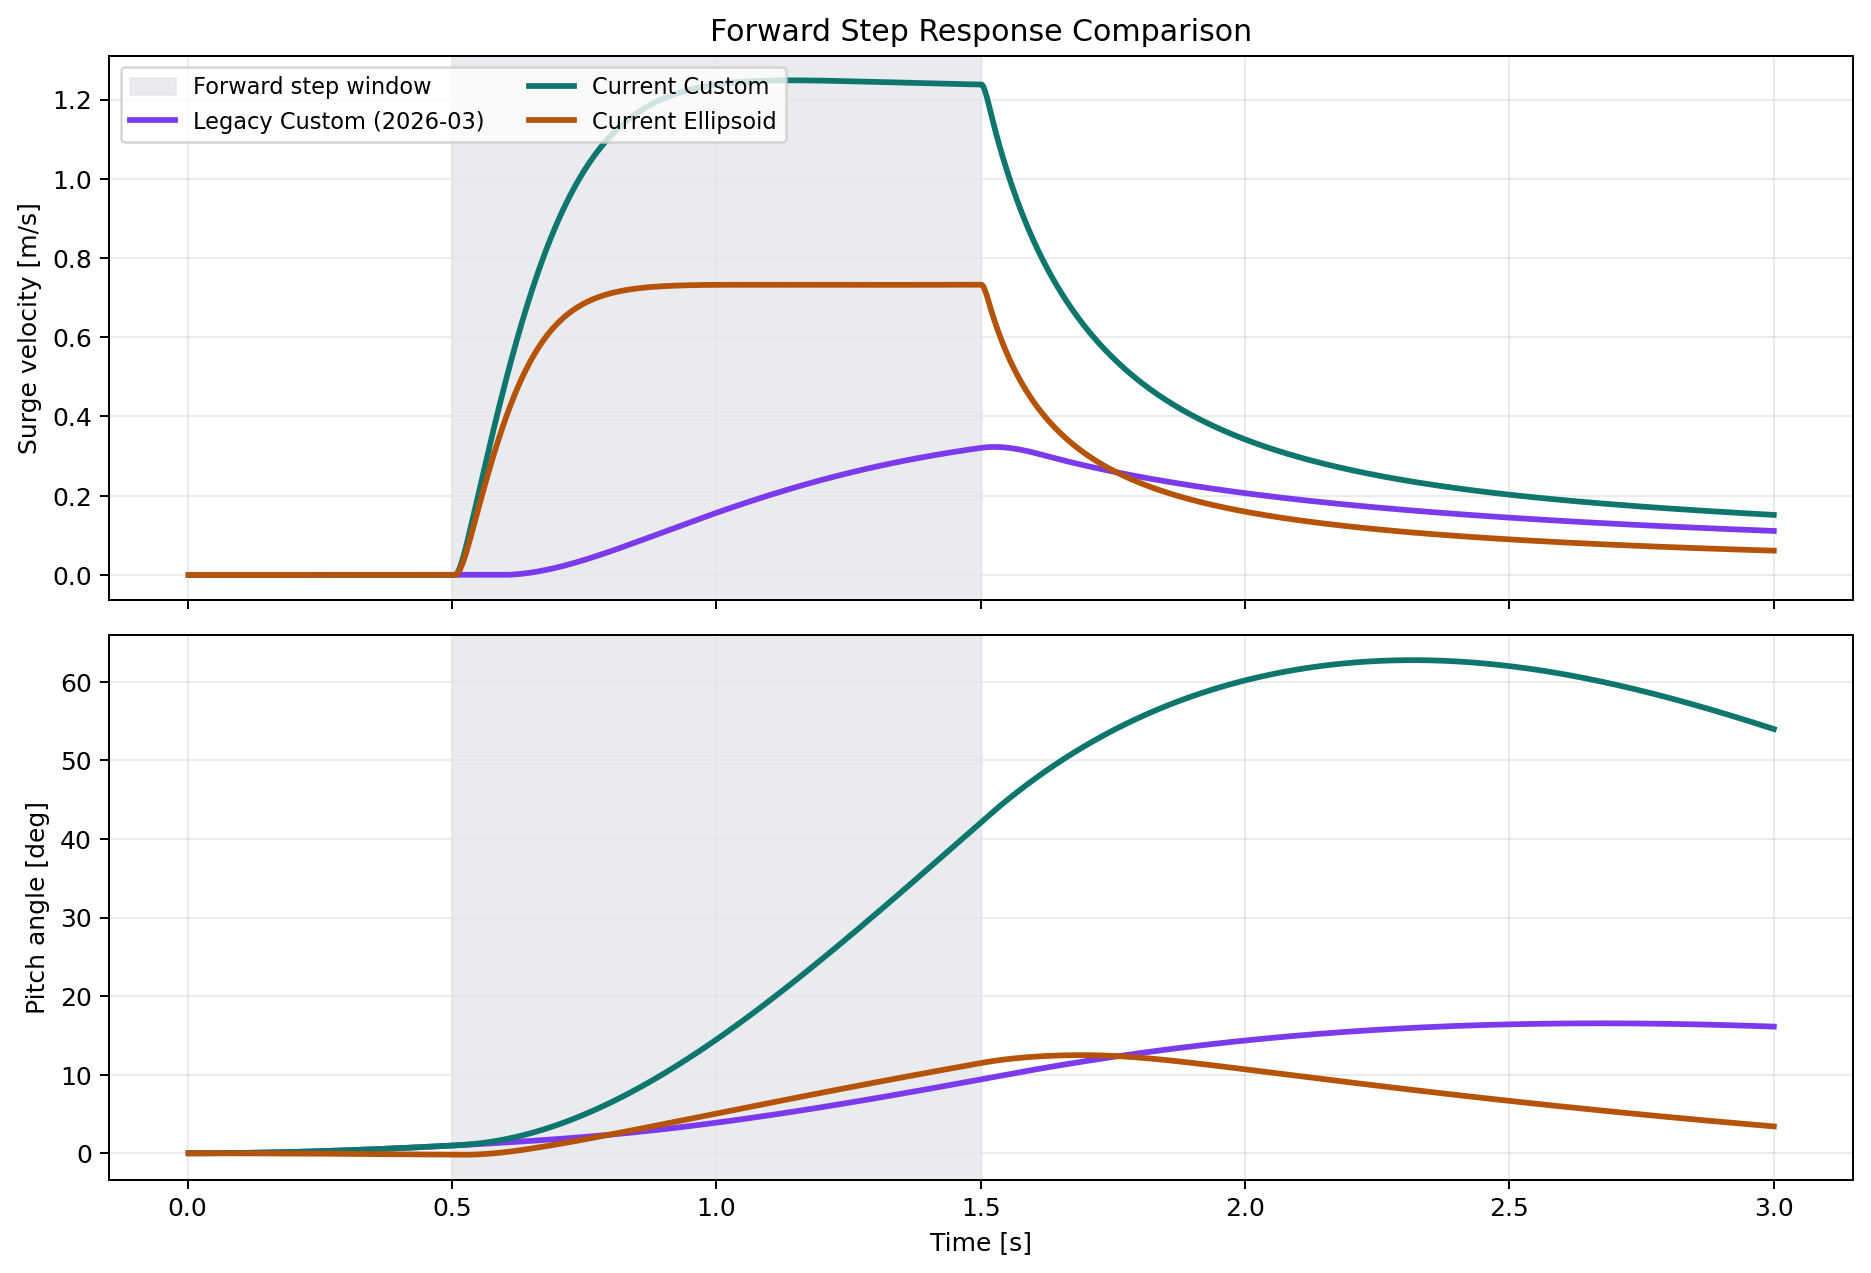
\includegraphics[width=0.96\linewidth]{figures/engine_forward_step_comparison.png}
  \caption{세 경로에 동일한 forward step을 재생한 결과. 위는 surge velocity, 아래는 pitch angle이다. 회색 음영은 입력이 실제로 들어간 구간이다.}
\end{figure}

이 그림에서 확인할 수 있는 핵심은 다음과 같다.

\begin{itemize}[leftmargin=2em]
  \item \textbf{Current Custom} 은 legacy 대비 peak surge가 약 \textbf{+299\%} 증가했지만, 동시에 peak pitch도 약 \textbf{+402\%} 증가하여 전진 명령이 자세 disturbance로 크게 연결된다.
  \item \textbf{Current Ellipsoid} 는 legacy 대비 peak surge가 약 \textbf{+134\%} 증가하면서도 peak pitch는 \textbf{12.51$^\circ$ $\rightarrow$ 12.49$^\circ$} 로 사실상 동일하다.
  \item 즉 \textbf{현재 ellipsoid 경로의 특별한 점}은 단순히 ``더 느리다''가 아니라, \textbf{지금 active thrust infrastructure를 유지한 채 pitch disturbance는 legacy 수준으로 억제한다}는 데 있다.
\end{itemize}

\subsection{Yaw step 비교}

\begin{figure}[htbp]
  \centering
  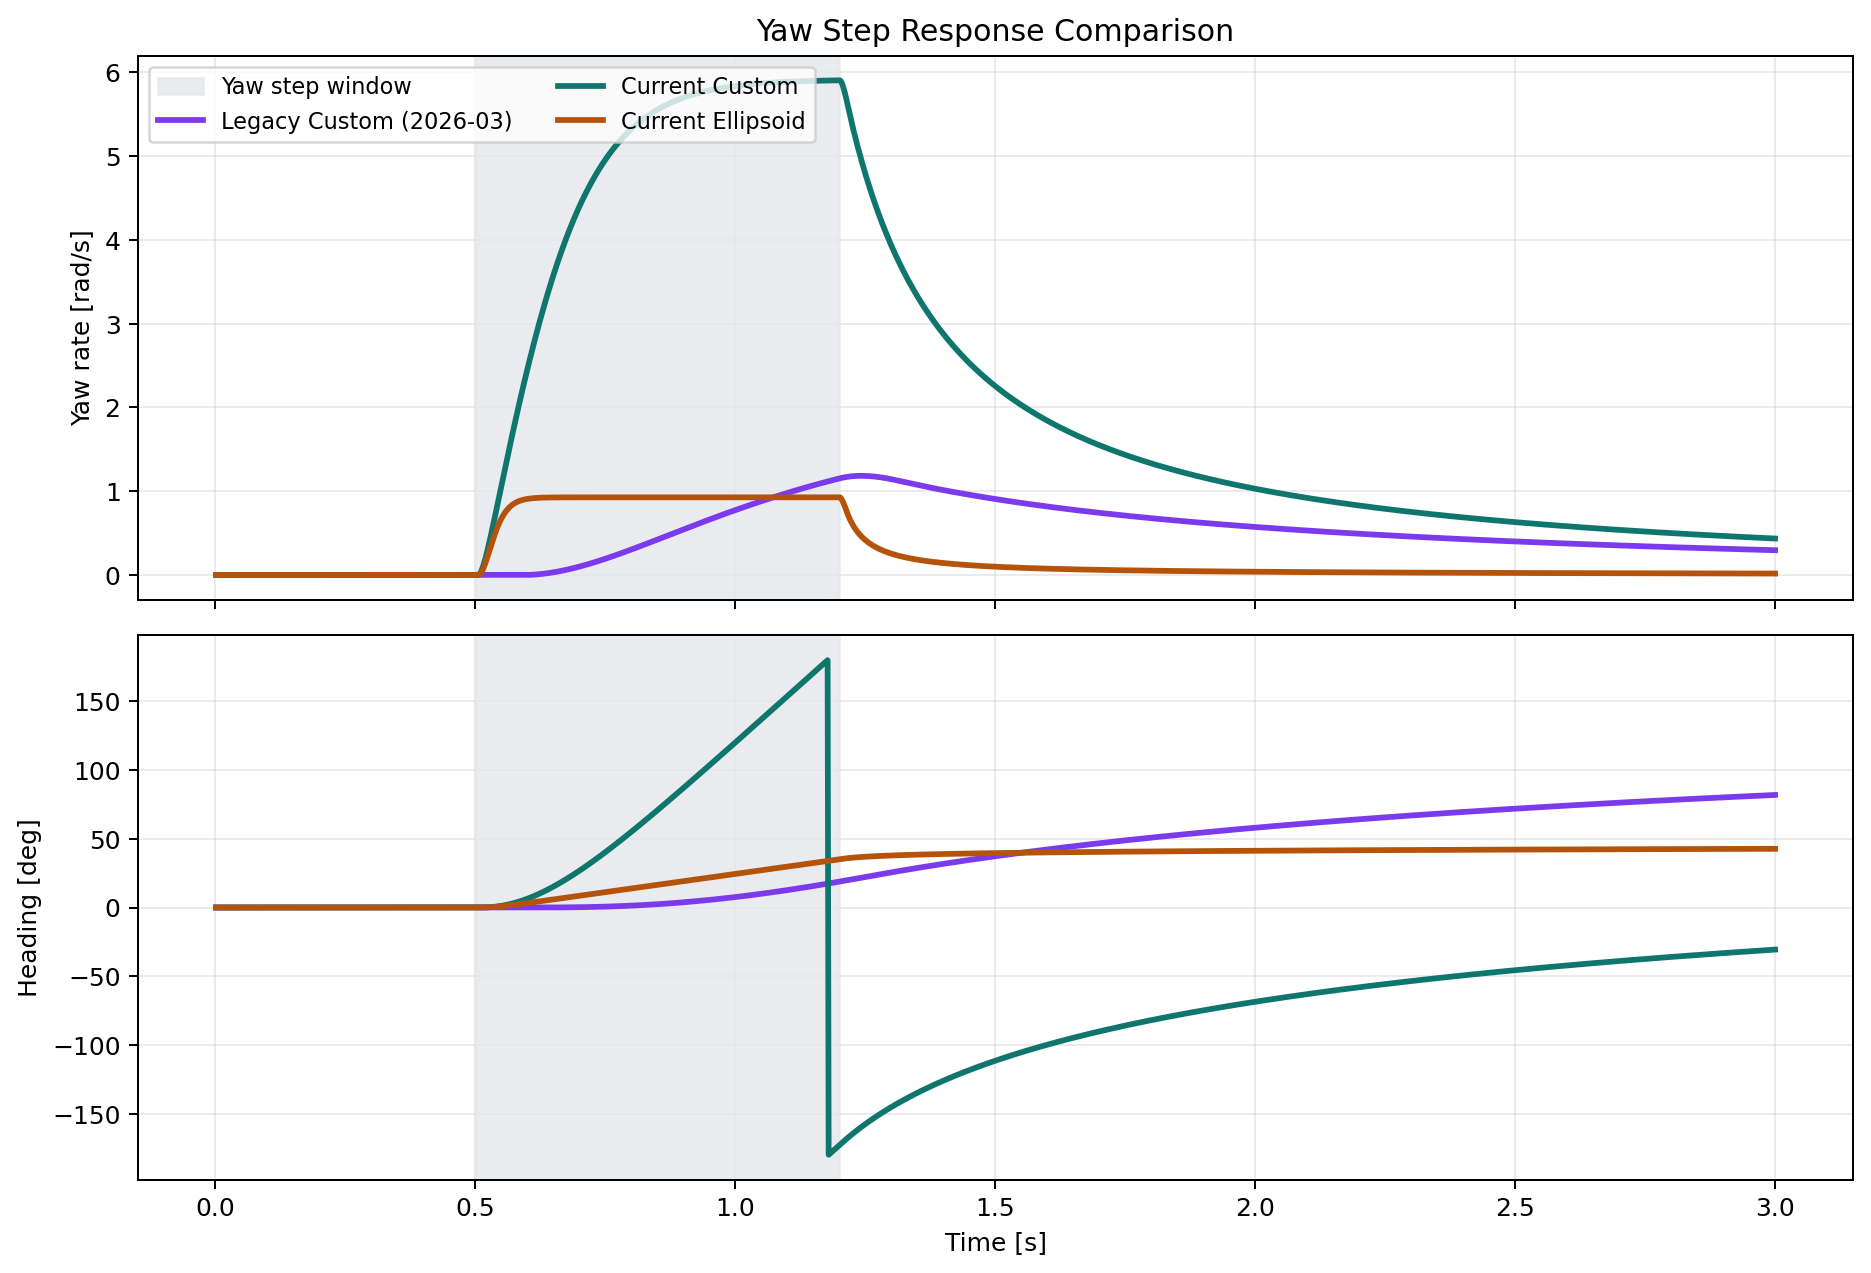
\includegraphics[width=0.96\linewidth]{figures/engine_yaw_step_comparison.png}
  \caption{세 경로에 동일한 yaw step을 재생한 결과. 위는 body yaw rate, 아래는 heading 누적값이다. 회색 음영은 입력 구간이다.}
\end{figure}

Yaw 응답에서는 차이가 더 분명하다.

\begin{itemize}[leftmargin=2em]
  \item \textbf{Current Custom} 은 peak yaw rate가 legacy 대비 약 \textbf{+1377\%} 증가했다. 대신 명령 해제 후 residual ratio는 \textbf{0.603 $\rightarrow$ 0.263} 으로 줄어들어 braking은 강하지만, 전체 응답이 매우 공격적으로 바뀌었다.
  \item \textbf{Current Ellipsoid} 는 peak yaw rate가 legacy 대비 약 \textbf{+132\%} 증가한 수준에 머문다. 반면 residual ratio는 \textbf{0.603 $\rightarrow$ 0.065} 로 크게 줄어들어, \textbf{회전 후 남는 꼬리 움직임은 세 경로 중 가장 작다}.
  \item \textbf{Current Ellipsoid vs Current Custom} 만 직접 비교하면, peak yaw rate는 약 \textbf{-84\%} 낮지만 residual ratio도 약 \textbf{-75\%} 낮다. 즉 ``느린 대신 매우 빨리 정리되는'' 응답이다.
\end{itemize}

\subsection{요약 메트릭과 특별한 부분}

\begin{figure}[htbp]
  \centering
  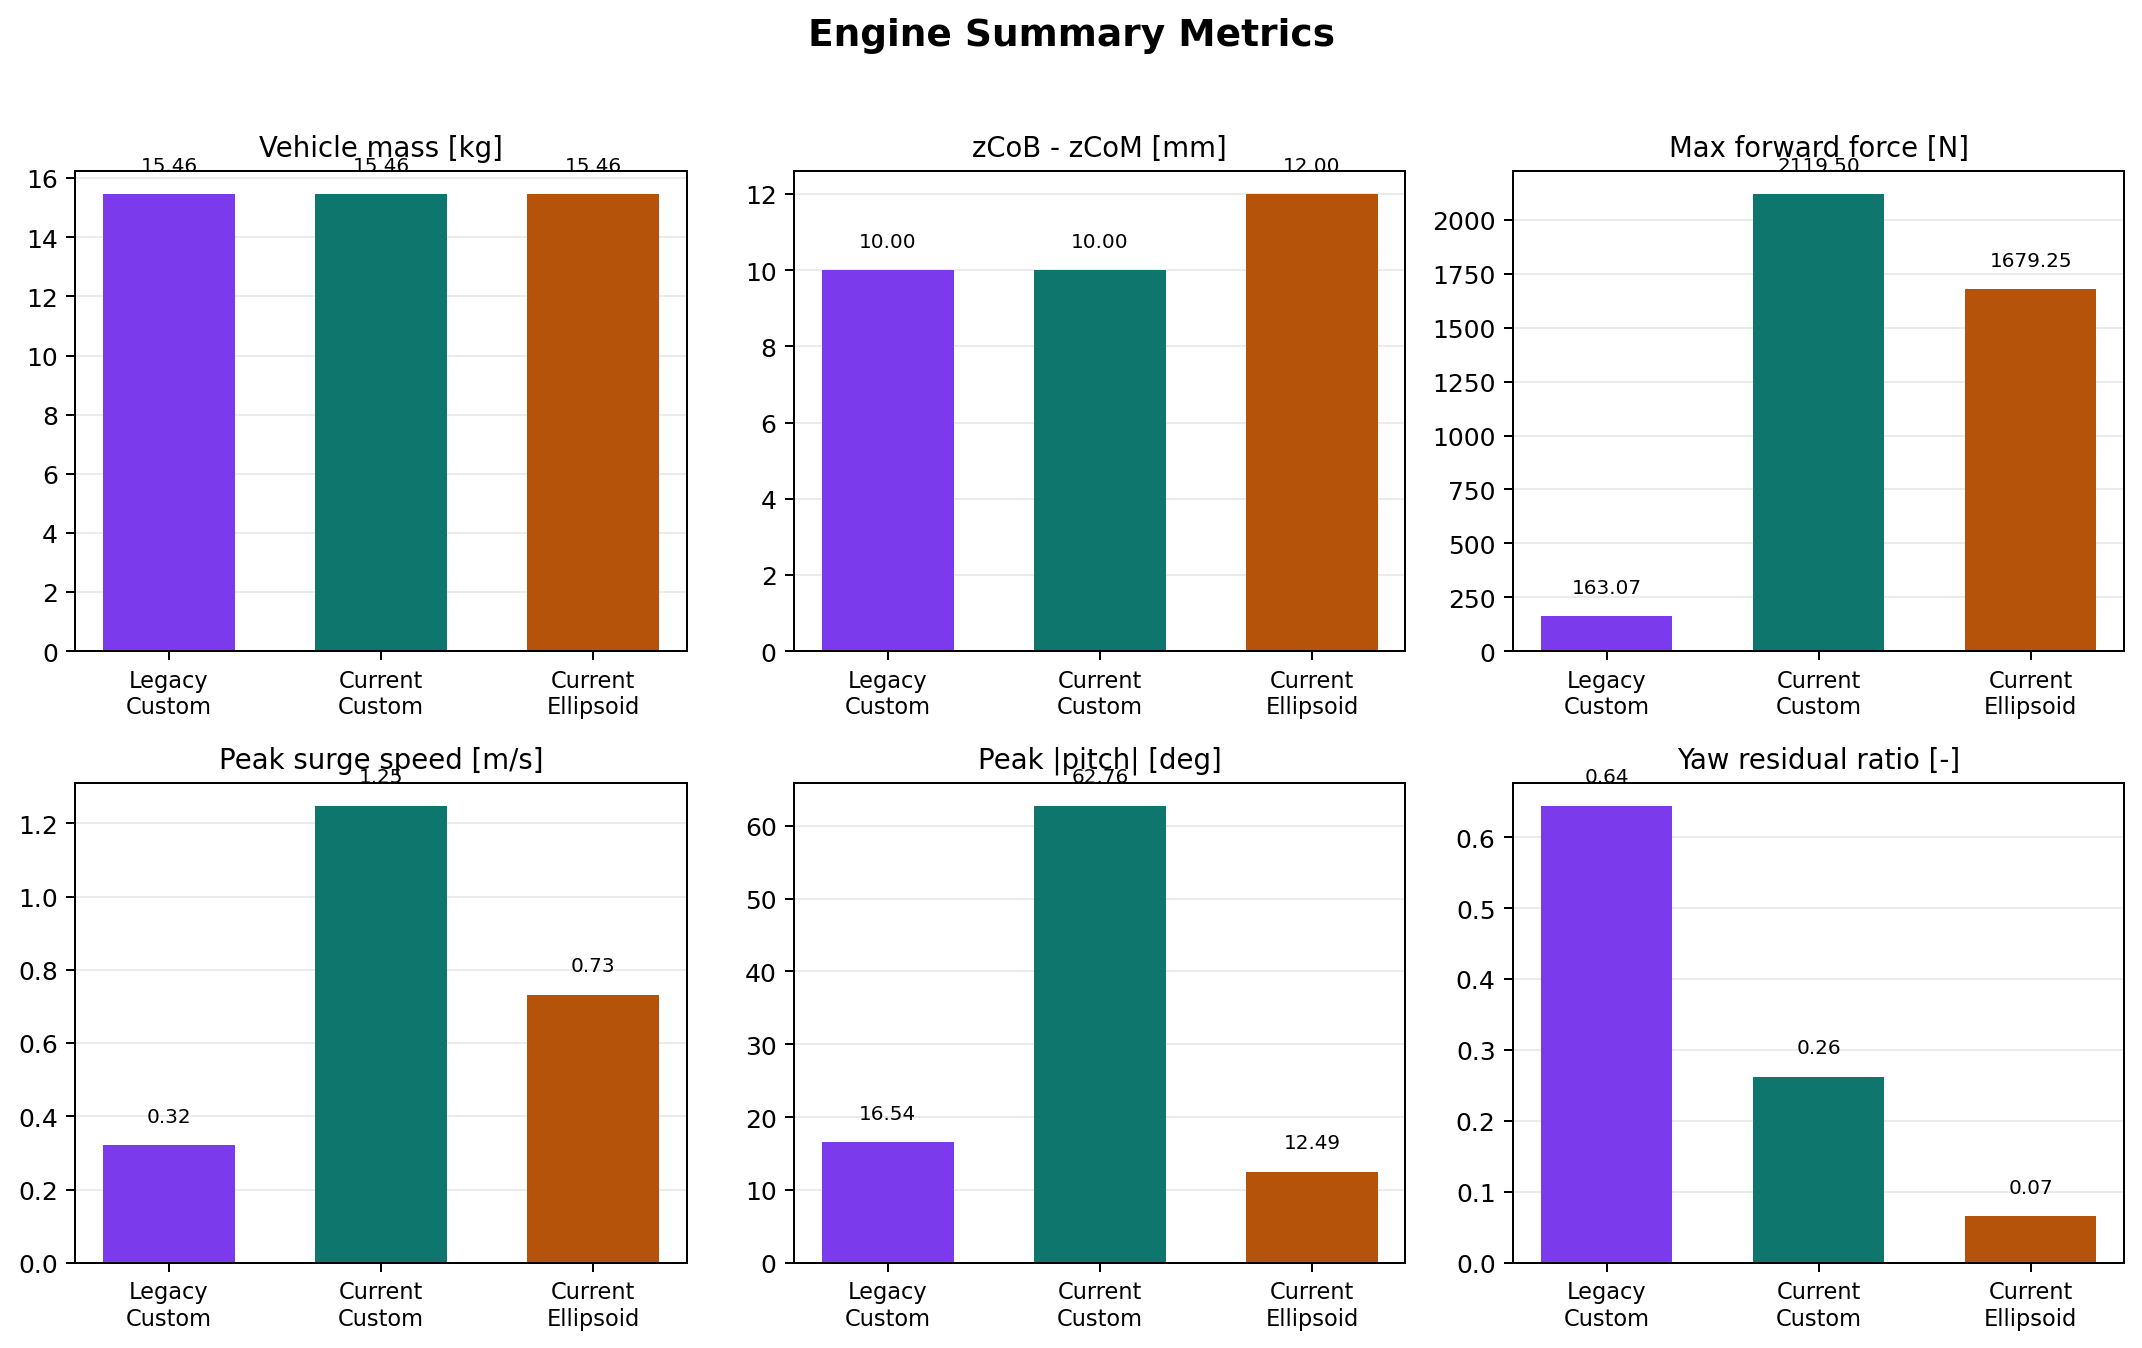
\includegraphics[width=0.98\linewidth]{figures/engine_summary_metrics.png}
  \caption{세 경로의 핵심 요약 메트릭. 질량, CoB--CoM 거리, 최대 전진 힘, peak surge, peak pitch, yaw residual ratio를 한 그림에서 비교한다.}
\end{figure}

이 그림이 보여주는 특별한 부분은 다음 세 가지다.

\begin{itemize}[leftmargin=2em]
  \item \textbf{지금 active custom 경로는 archived legacy보다 매우 공격적으로 변했다.} forward force와 yaw moment가 각각 약 12배 수준으로 커졌고, 그 대가로 pitch coupling이 매우 커졌다.
  \item \textbf{현재 ellipsoid 경로는 active custom보다 전진/회전 authority가 작지만, pitch disturbance와 residual yaw는 훨씬 작다.} 따라서 ``조이스틱 추종은 유지하되 흔들림은 줄이고 싶은'' 목표에 더 가까운 baseline으로 볼 수 있다.
  \item \textbf{이 차이는 순수하게 엔진 하나만의 차이가 아니다.} 현재 active scene은 질량(15.46 kg), CoB 설정, actuator 범위, 전역 thruster scale이 legacy와 모두 달라졌기 때문이다. 따라서 문서에서 반드시 ``engine difference'' 와 ``full runtime tuning difference'' 를 함께 말해야 한다.
\end{itemize}

\section{ROS bag 기반 모드 경로 검증}

이 절의 목적은 단순한 single-axis step response가 아니라, \textbf{실제 operator가 조이스틱으로 주는 복합 기동}에 대해 현재 simulator가 어떻게 움직이는지를 보여주는 것이다. 따라서 이번 측정에서는 ``전진''만 본 것이 아니라,

\begin{quote}
\small
전진 $\rightarrow$ 약 90$^\circ$ 회전 $\rightarrow$ 우측 이동
\end{quote}

으로 이어지는 L자 경로를 \textbf{MANUAL, STABILIZE, ALT\_HOLD, POSHOLD} 네 모드에서 모두 수행했다. 또한 이 시퀀스를 \textbf{current custom} 과 \textbf{current ellipsoid} 두 active engine 경로에 동일하게 재생해, 실제 \code{ros2 bag} 기반으로 비교했다.

\subsection{측정 설정}

측정 절차는 다음과 같다.

\begin{enumerate}[leftmargin=2em]
  \item \code{document/run\_actual\_mode\_path\_measurement.sh custom custom} 으로 \textbf{current custom} 경로를 측정했다.
  \item \code{document/run\_actual\_mode\_path\_measurement.sh ellipsoid ellipsoid} 으로 \textbf{current ellipsoid} 경로를 측정했다.
  \item 두 경우 모두 \code{start\_sitl\_mujoco\_mj311.sh --ros2 --sitl-no-rebuild} 경로로 simulator를 기동했고, 내부 \code{/mavros/*} service 와 topic surface 를 사용했다.
  \item \code{document/measure\_mavros\_mode\_path\_sequence.py} 가 \code{/mavros/set\_mode}, \code{/mavros/cmd/arming}, \code{/mavros/rc/override} 를 호출해 네 모드의 동일한 L자 경로 명령을 넣었다.
  \item \code{/mavros/local\_position/odom}, \code{/mavros/imu/data}, \code{/depth}, \code{/mavros/state}, \code{/measurement/phase} 를 \code{ros2 bag} 으로 기록하고, \code{document/analyze\_mode\_path\_bag.py} 가 3D 궤적과 정량 메트릭을 생성했다.
\end{enumerate}

이번 측정에서 사용한 실제 bag 디렉터리는 다음과 같다.

\begin{itemize}[leftmargin=2em]
  \item \code{document/measurements/mode\_path\_custom\_20260403\_190110}
  \item \code{document/measurements/mode\_path\_ellipsoid\_20260403\_190412}
\end{itemize}

\subsection{3D 경로와 엔진 간 차이}

\begin{figure}[htbp]
  \centering
  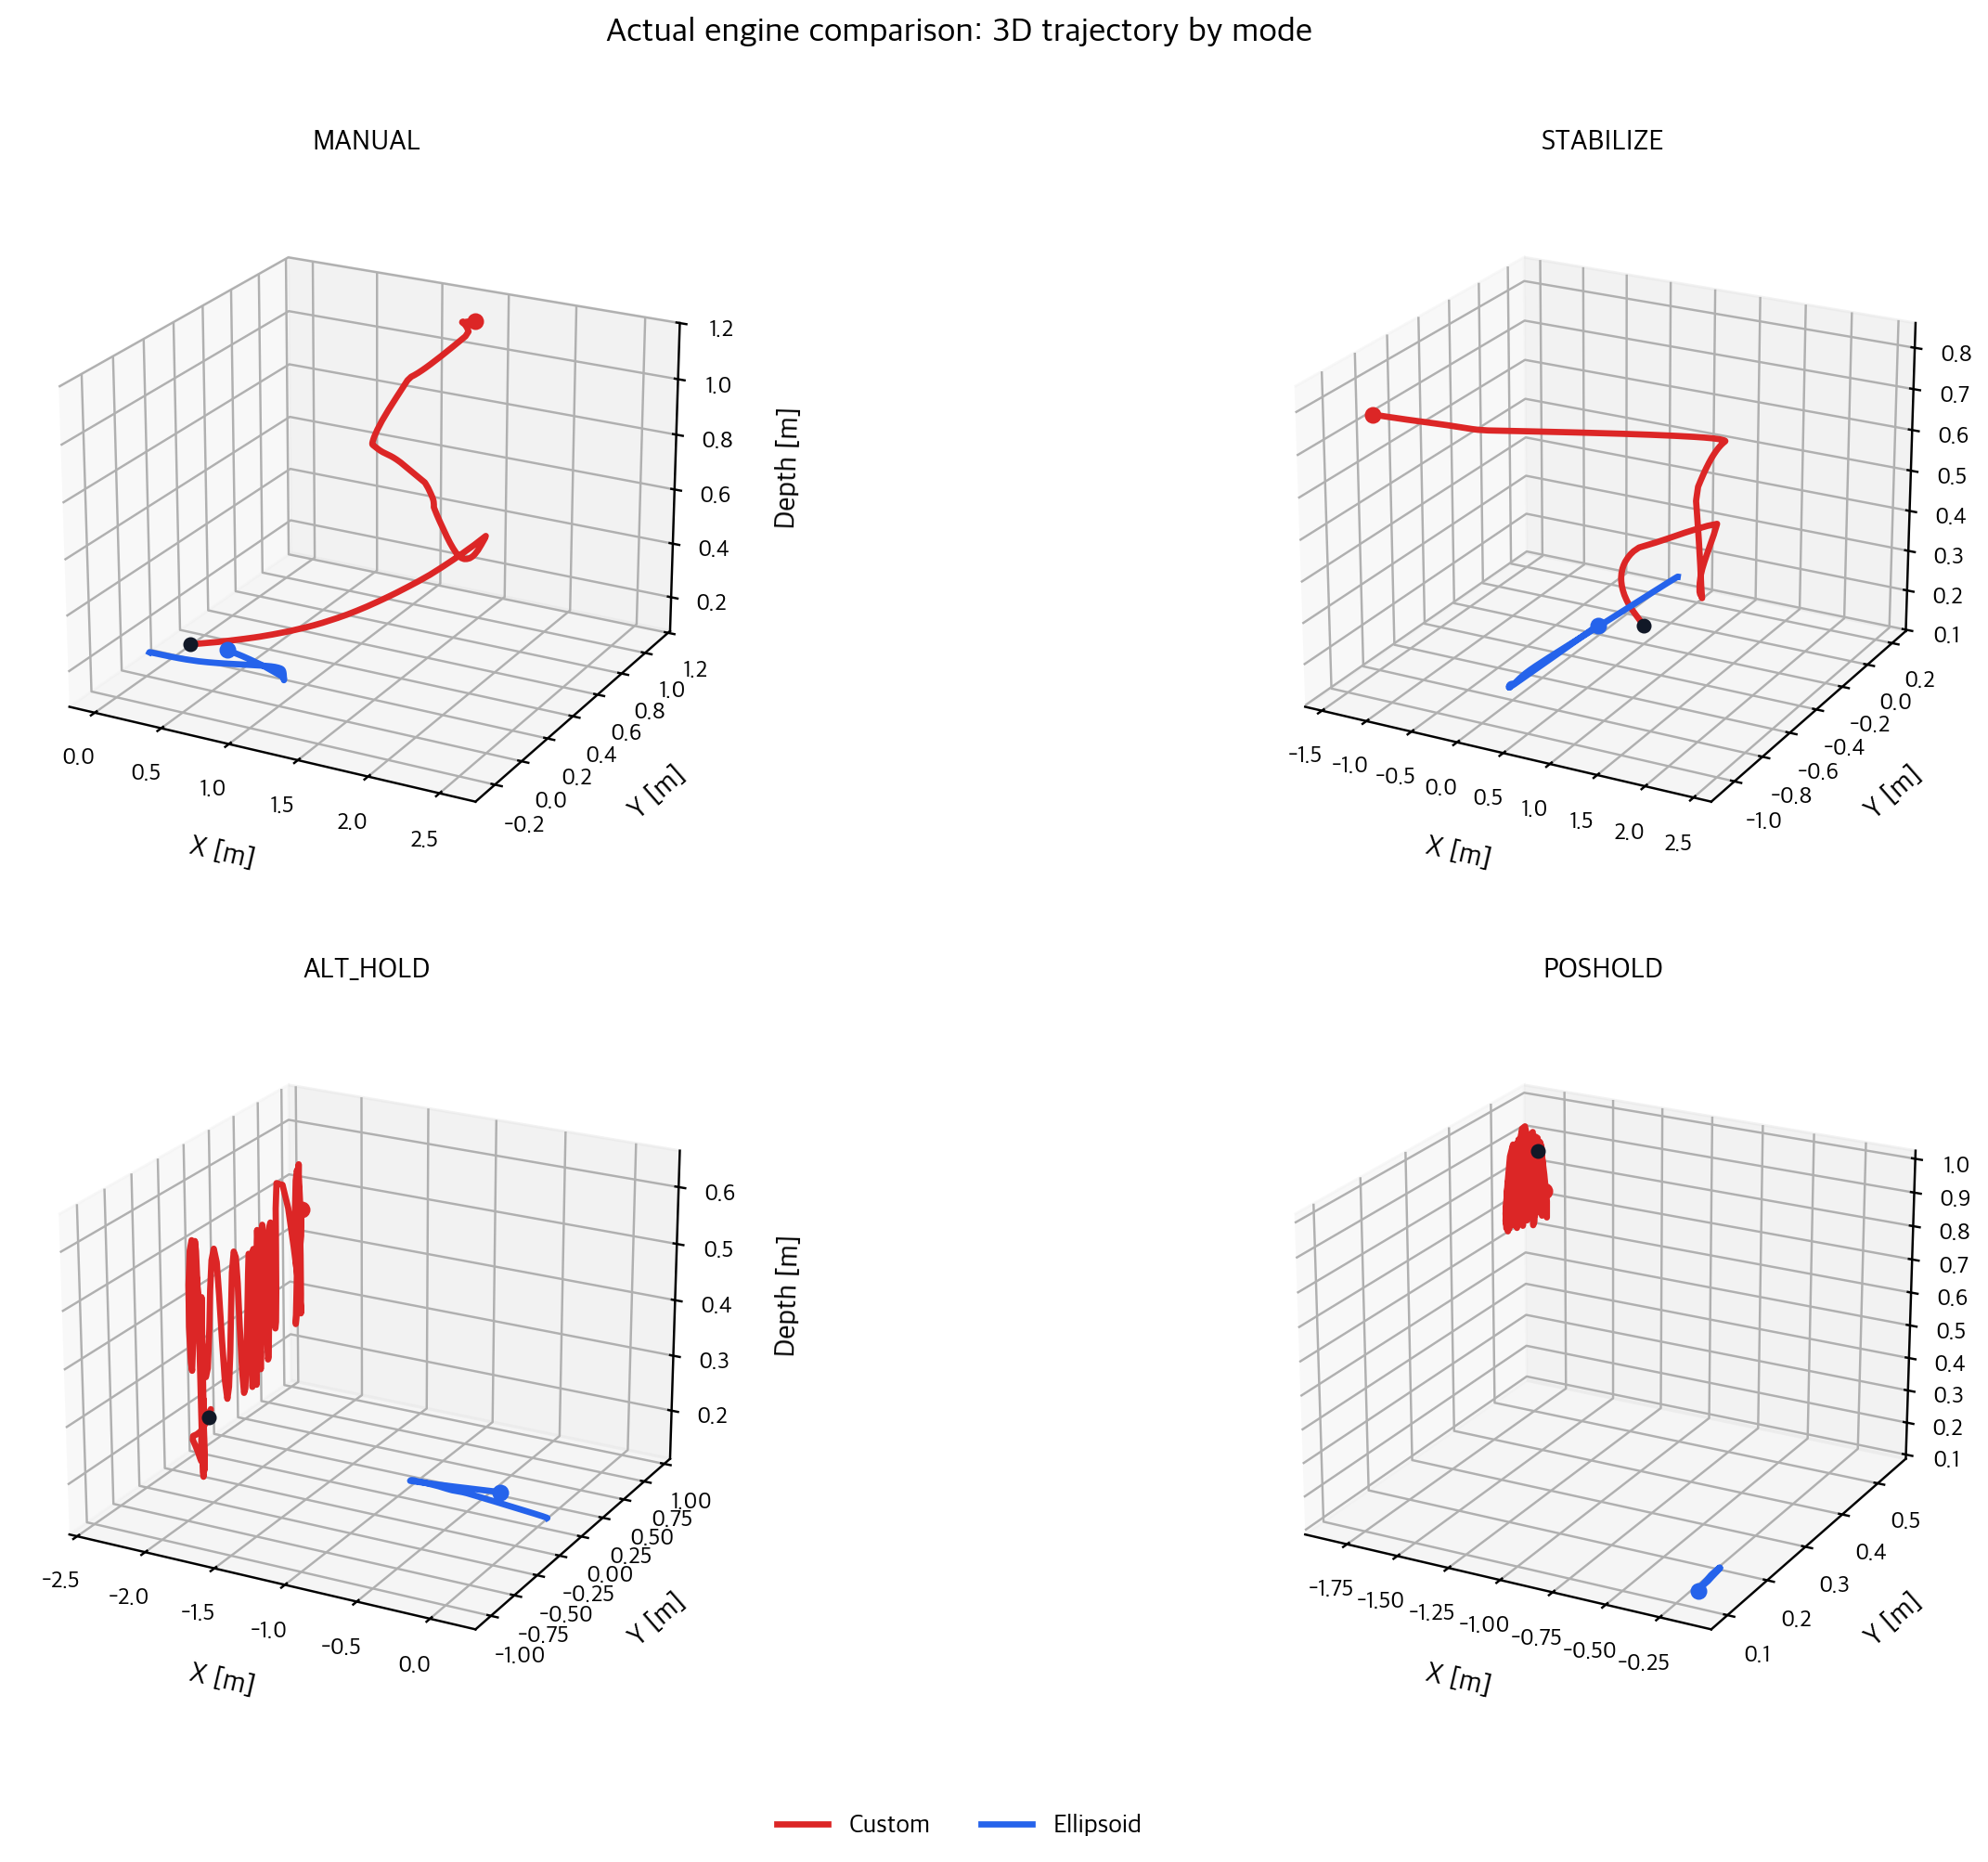
\includegraphics[width=0.96\linewidth]{figures/engine_mode_path_3d_comparison.png}
  \caption{실제 3D trajectory 기준 engine comparison. 각 subplot은 하나의 mode를 나타내며, 빨강은 current custom, 파랑은 current ellipsoid 다. 즉 ``전진 $\rightarrow$ 90$^\circ$ turn $\rightarrow$ 우측 이동'' 전체가 \textbf{하나의 연속 경로}로 어떻게 누적되는지를 직접 비교한 그림이다.}
\end{figure}

\begin{figure}[htbp]
  \centering
  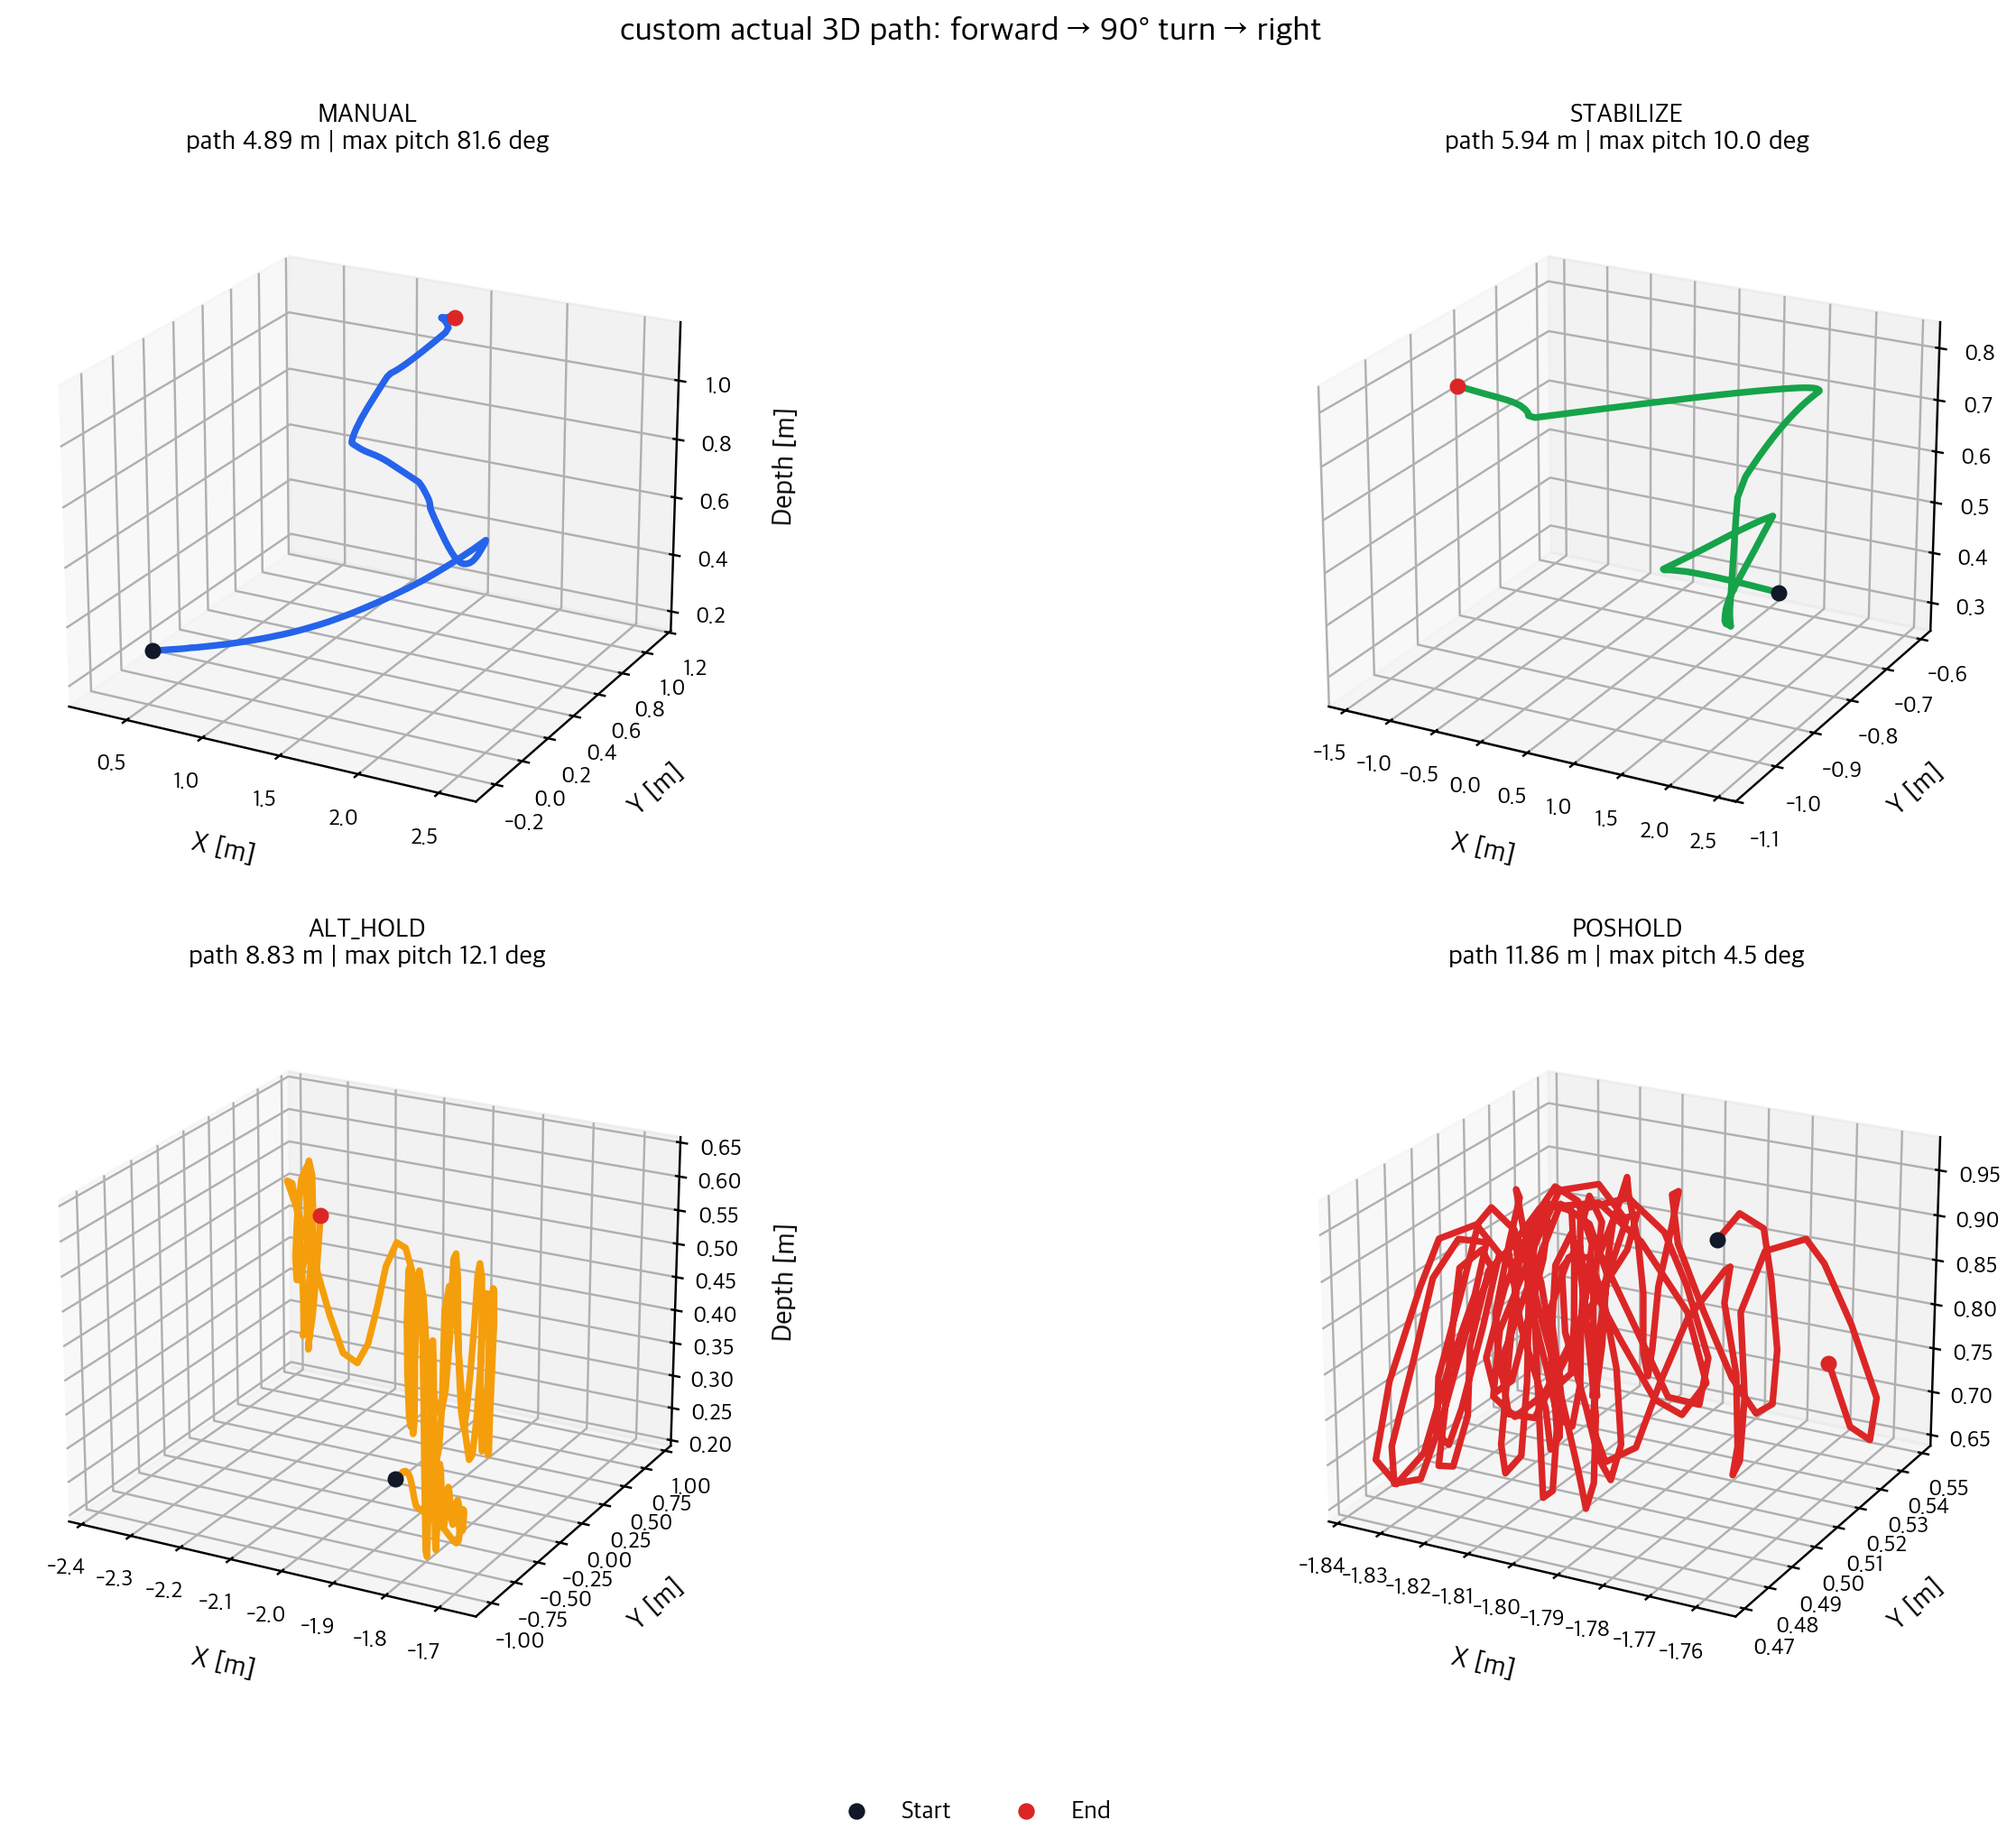
\includegraphics[width=0.96\linewidth]{figures/actual_custom_mode_path_3d.png}
  \caption{Current custom 의 mode별 실제 3D trajectory. segment를 분리하지 않고 full path만 그려, 하나의 모드에서 경로가 얼마나 길게 늘어지거나 회전 후 drift를 남기는지를 읽을 수 있게 했다.}
\end{figure}

\begin{figure}[htbp]
  \centering
  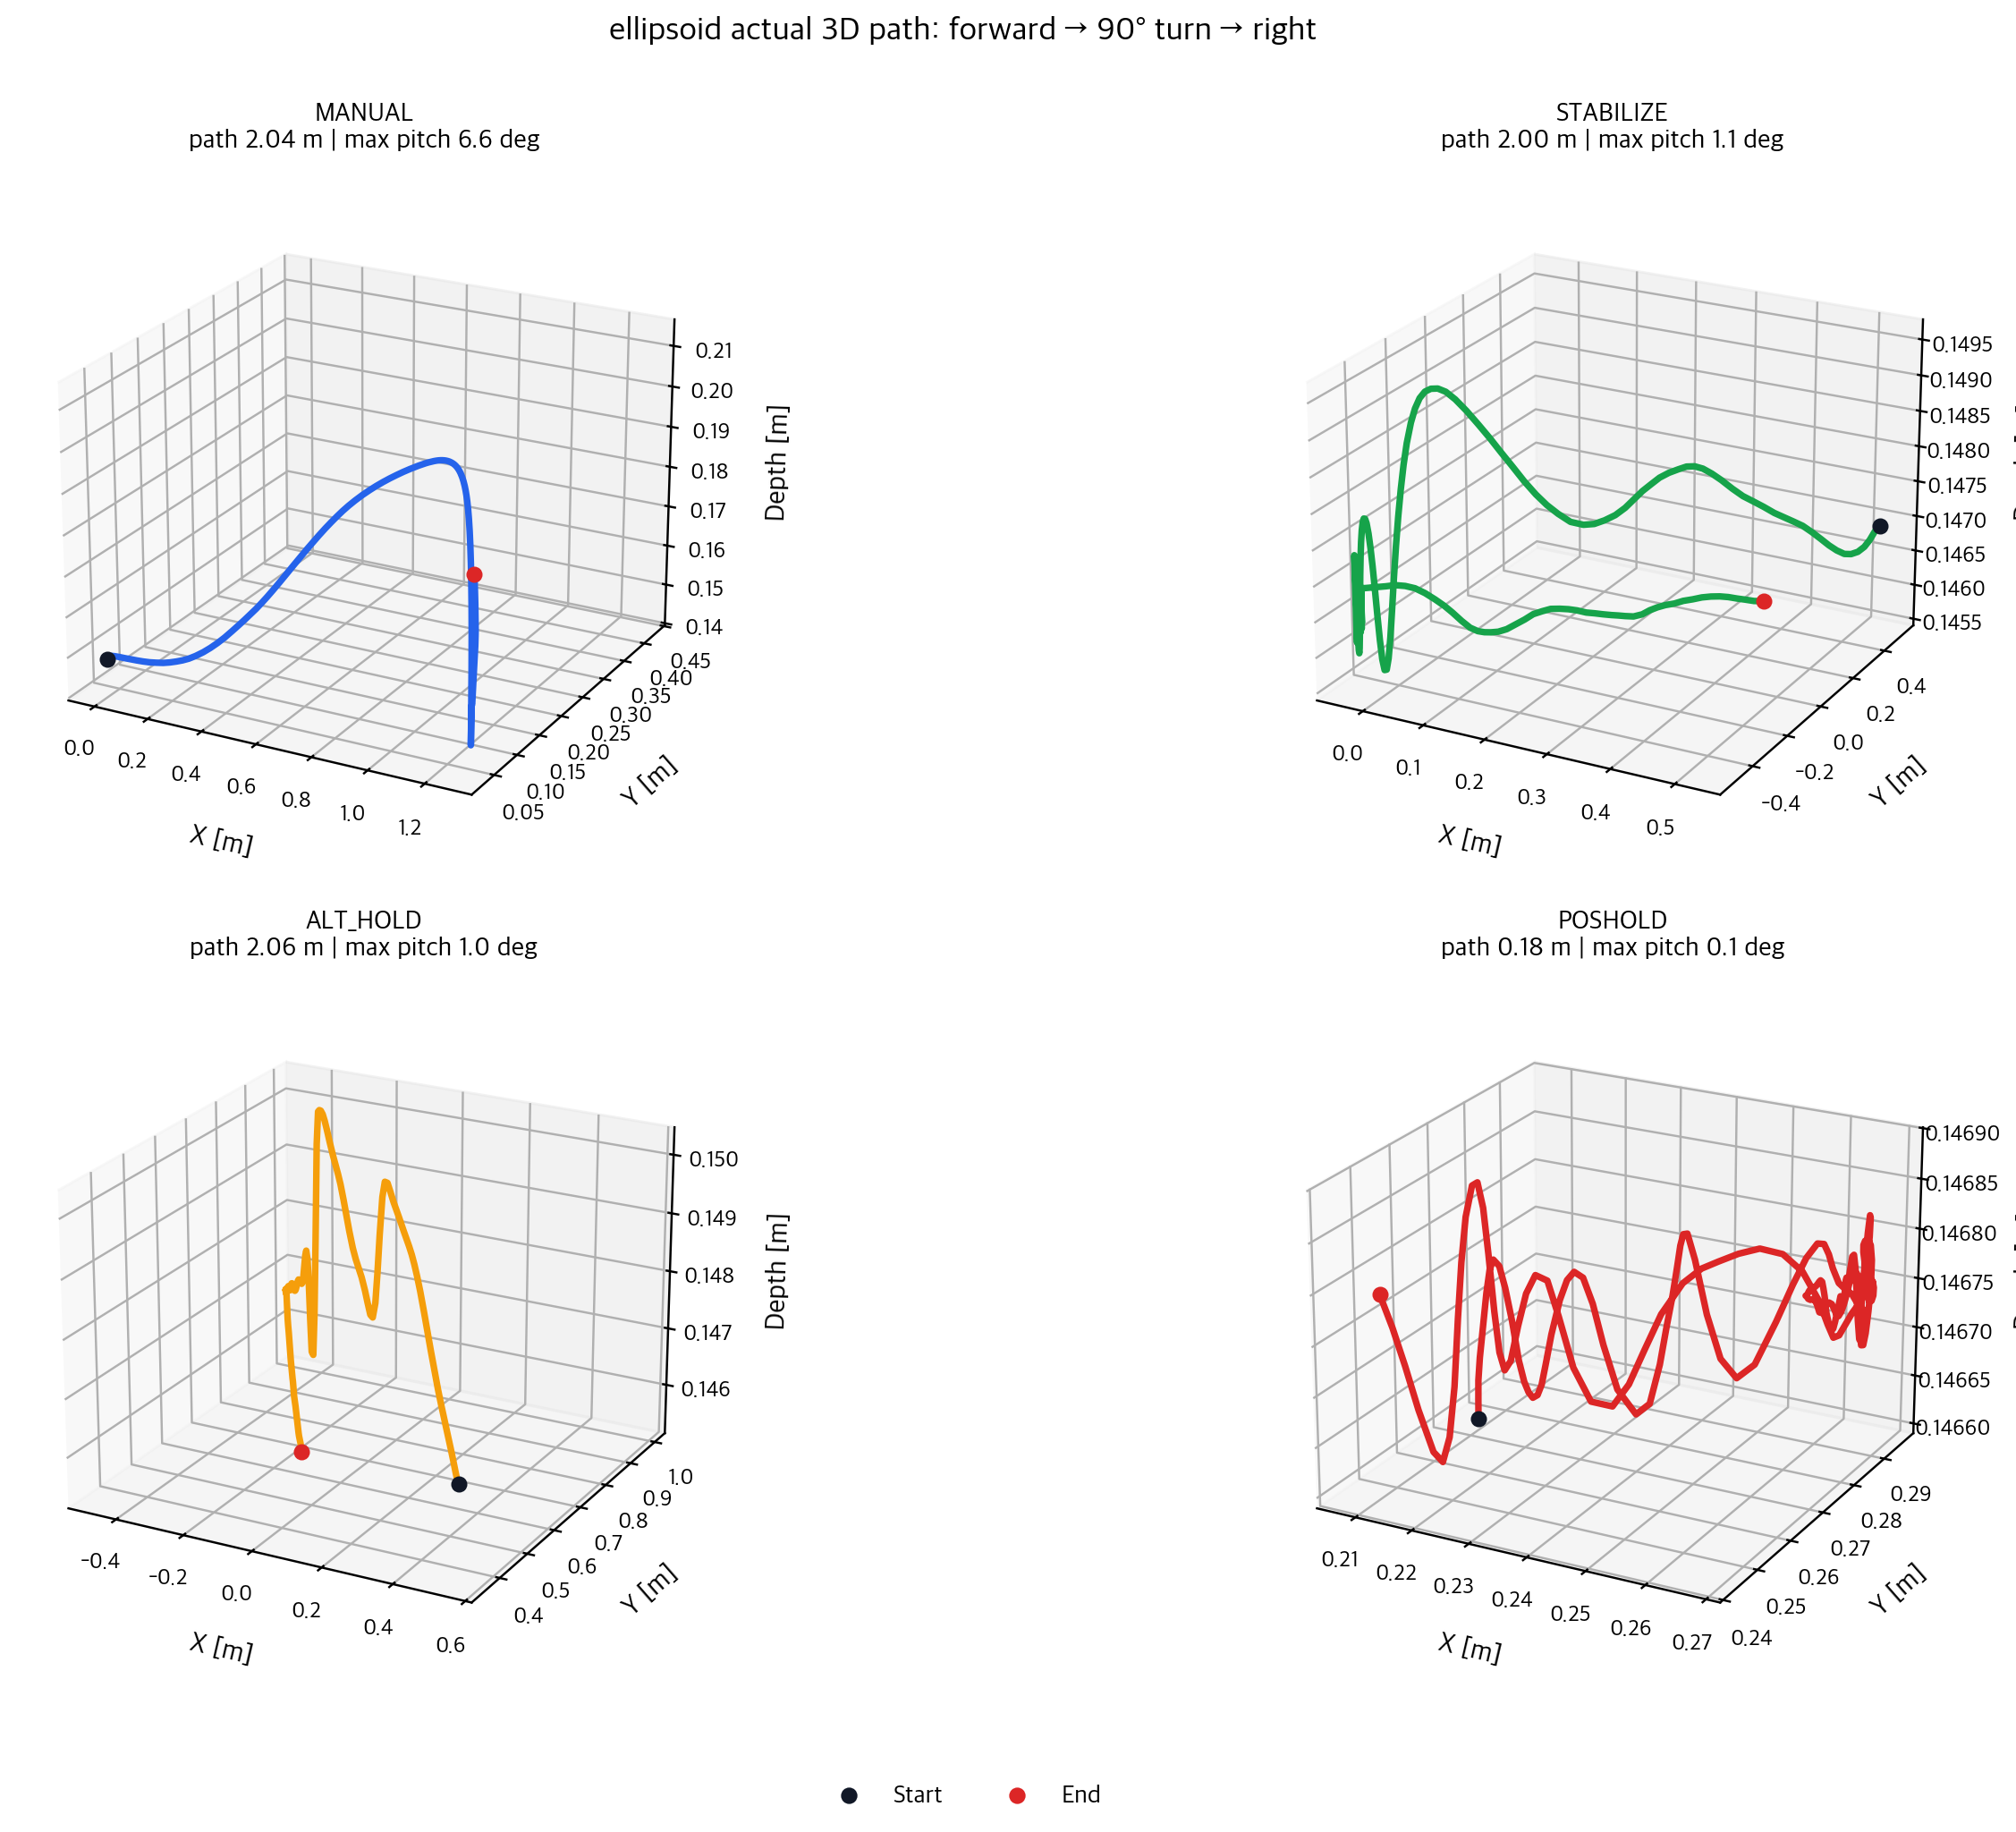
\includegraphics[width=0.96\linewidth]{figures/actual_ellipsoid_mode_path_3d.png}
  \caption{Current ellipsoid 의 mode별 실제 3D trajectory. current custom 보다 path length가 짧고 종료점이 빠르게 정리되는 경향이 더 분명하게 보인다.}
\end{figure}

\begin{figure}[htbp]
  \centering
  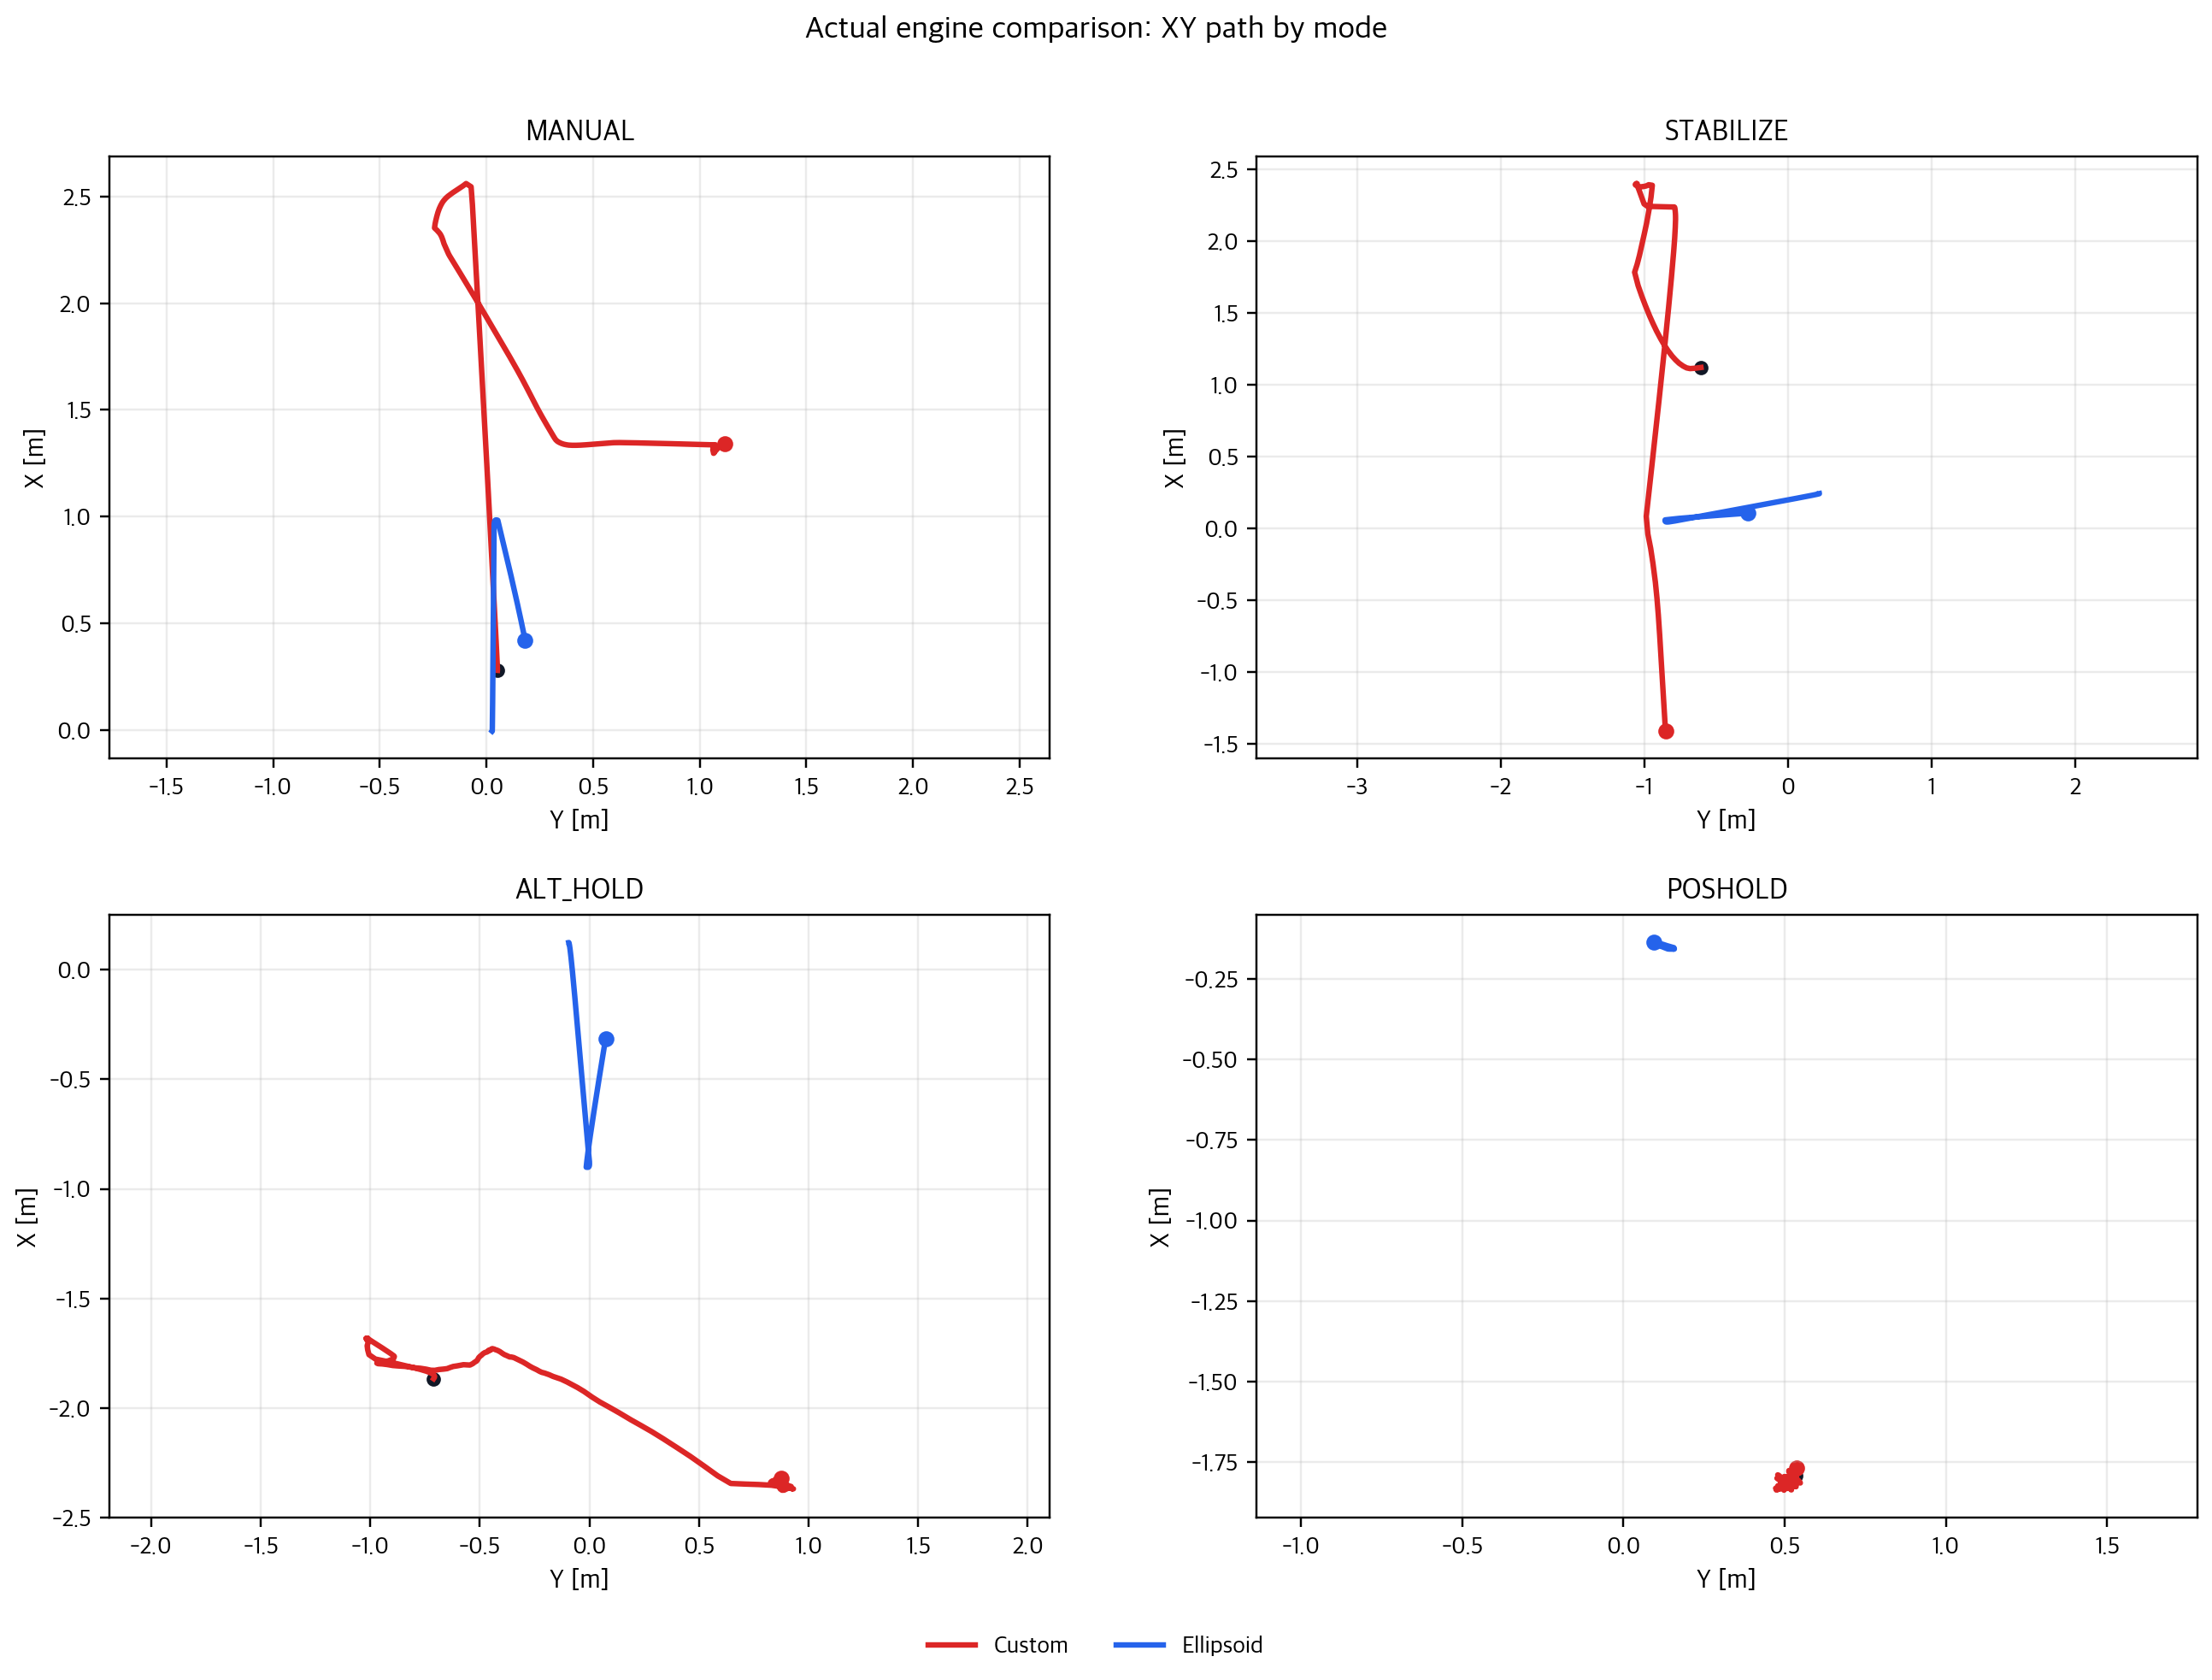
\includegraphics[width=0.96\linewidth]{figures/engine_mode_path_xy_comparison.png}
  \caption{실제 XY 궤적 기준 engine comparison. 위 3D 경로의 평면 투영으로, L자 경로의 형상과 drift tail 을 더 쉽게 읽기 위한 그림이다.}
\end{figure}

이 세 그림이 보여주는 가장 중요한 차이는 다음과 같다.

\begin{itemize}[leftmargin=2em]
  \item \textbf{Current custom} 은 조이스틱에 대해 authority가 크지만, MANUAL과 STABILIZE에서 overshoot와 drift가 크다. 특히 MANUAL에서는 90$^\circ$ turn 명령이 실제로는 \textbf{149.5$^\circ$} 까지 진행됐고, 최대 pitch는 \textbf{81.6$^\circ$} 까지 상승했다.
  \item \textbf{Current ellipsoid} 는 같은 입력에서 이동량은 더 작지만 path가 훨씬 정리된다. MANUAL turn은 \textbf{-96.8$^\circ$} 로 90$^\circ$ 명령에 가깝고, 최대 pitch는 \textbf{5.46$^\circ$} 에 그친다.
  \item \textbf{POSHOLD} 차이는 가장 극적이다. current custom 은 forward/right leg 자체는 거의 형성되지 않는데도 전체 path length가 \textbf{11.86 m} 에 달했고, current ellipsoid 는 \textbf{0.145 m} 로 매우 짧게 정리됐다. 즉 위치 유지 관점에서 current ellipsoid 가 훨씬 안정적이다.
\end{itemize}

\subsection{모드별 정량 비교}

\begin{figure}[htbp]
  \centering
  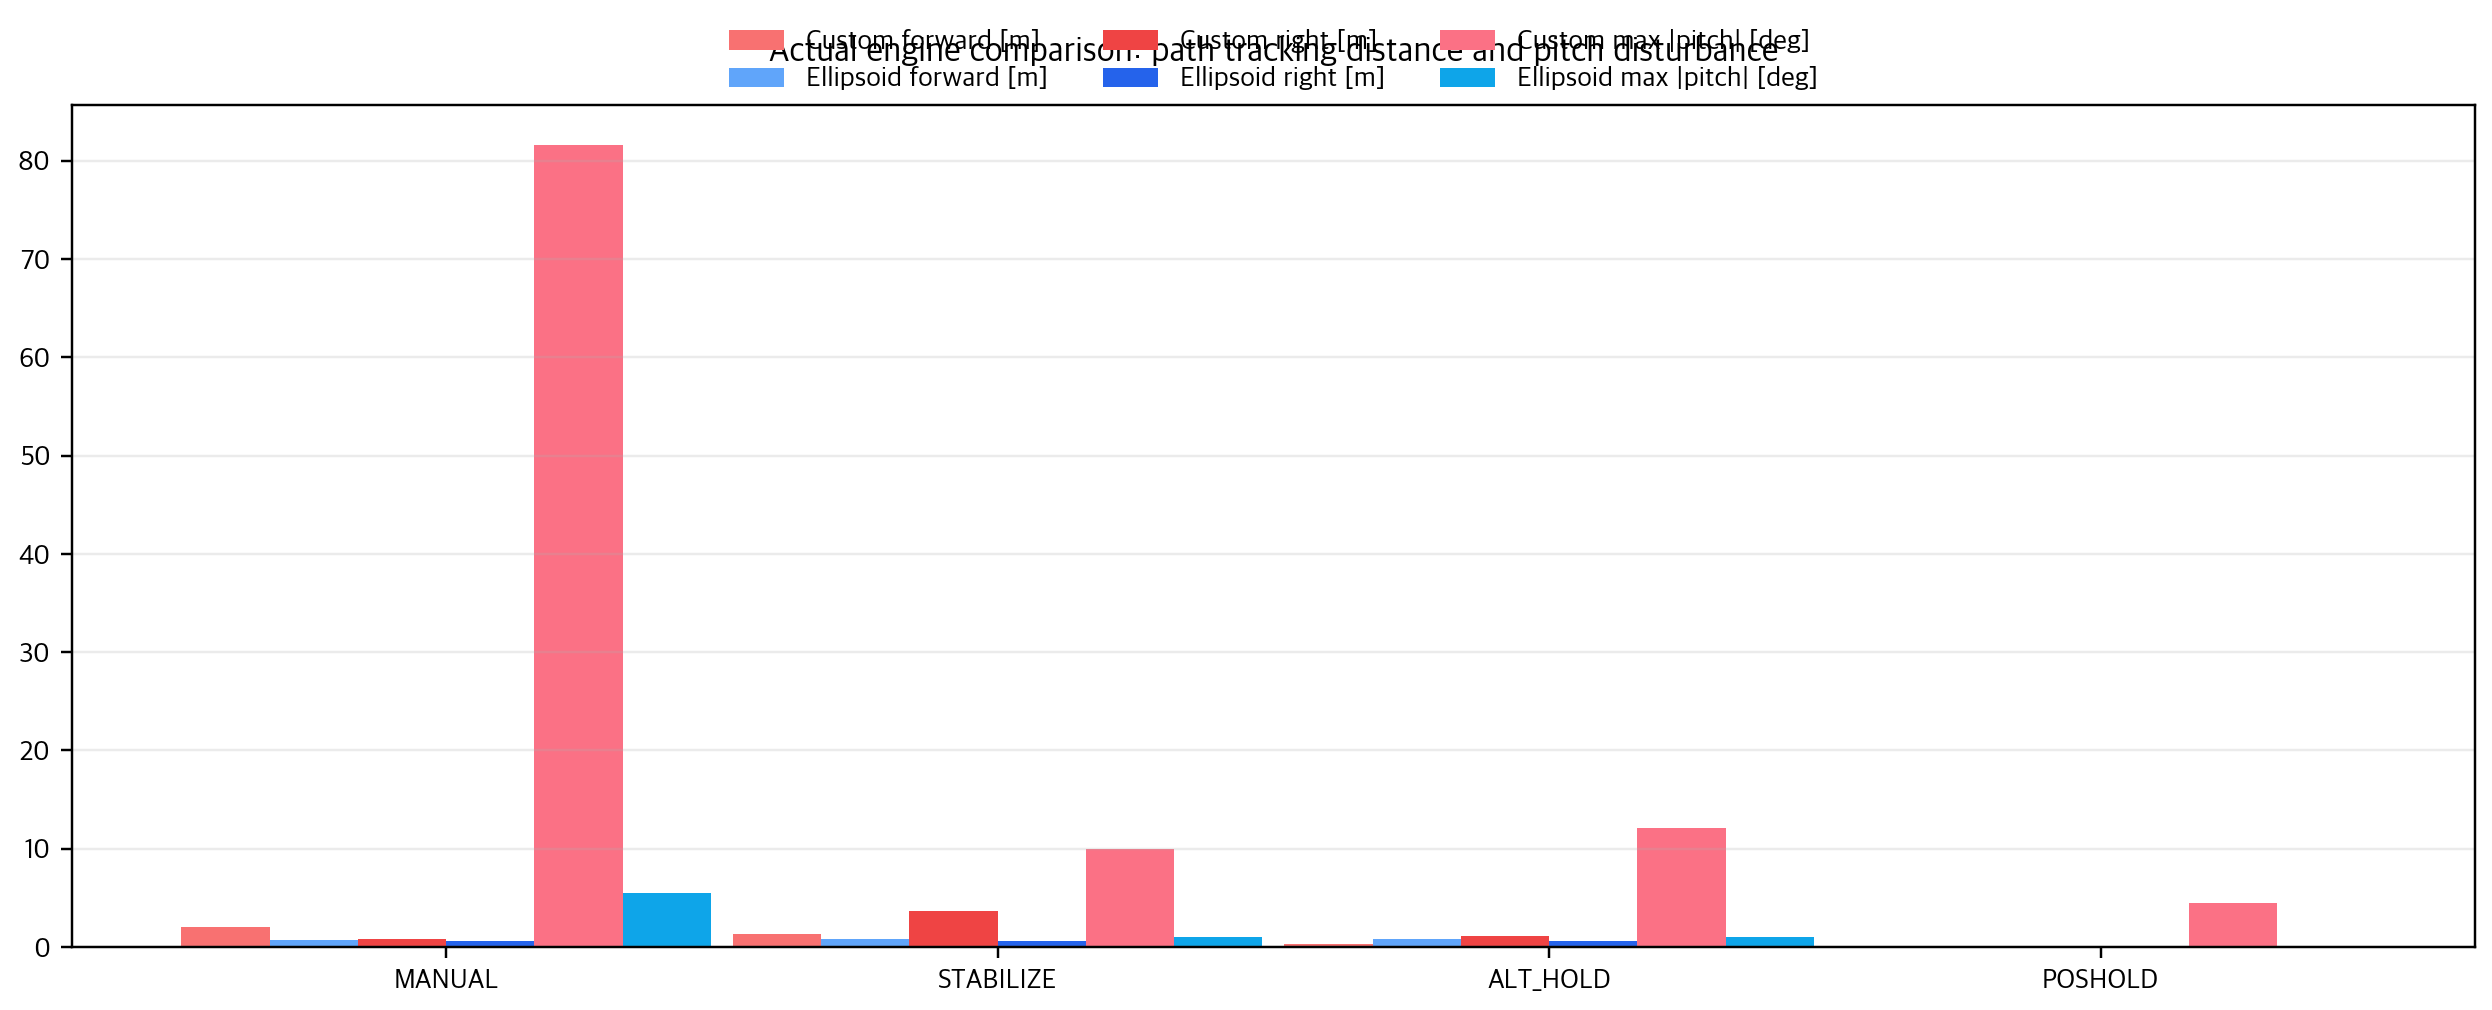
\includegraphics[width=0.96\linewidth]{figures/engine_mode_path_metrics.png}
  \caption{실제 모드 경로의 정량 메트릭 비교. forward leg 거리, right leg 거리, 최대 pitch disturbance를 mode별로 custom/ellipsoid 에 대해 함께 나타낸다.}
\end{figure}

\begingroup
\begin{center}
\scriptsize
\setlength{\tabcolsep}{3.5pt}
\begin{tabularx}{\linewidth}{>{\raggedright\arraybackslash}p{0.13\linewidth}>{\raggedright\arraybackslash}p{0.12\linewidth}>{\raggedright\arraybackslash}p{0.11\linewidth}>{\raggedright\arraybackslash}p{0.11\linewidth}>{\raggedright\arraybackslash}p{0.11\linewidth}>{\raggedright\arraybackslash}p{0.11\linewidth}Y}
\toprule
Mode & Engine & Forward [m] & Turn [deg] & Right [m] & Path [m] & 특별한 점 \\
\midrule
MANUAL & Custom & 2.015 & 149.5 & 0.817 & 4.887 & 명령 대비 turn overshoot가 매우 크고 pitch disturbance가 큼 \\
MANUAL & Ellipsoid & 0.758 & -96.8 & 0.578 & 1.626 & 이동량은 작지만 90$^\circ$ turn 과 궤적이 훨씬 정리됨 \\
STABILIZE & Custom & 1.351 & -75.4 & 3.652 & 5.944 & 자세 안정화가 켜져도 right leg overshoot가 매우 큼 \\
STABILIZE & Ellipsoid & 0.840 & -76.0 & 0.577 & 1.688 & turn 각도는 비슷하지만 drift와 pitch가 매우 작음 \\
ALT\_HOLD & Custom & 0.354 & -66.2 & 1.119 & 8.829 & depth hold 중에도 path가 길게 늘어지며 pitch disturbance가 남음 \\
ALT\_HOLD & Ellipsoid & 0.792 & -69.8 & 0.593 & 1.635 & ALT\_HOLD에서도 훨씬 짧고 안정된 경로 형성 \\
POSHOLD & Custom & 0.045 & -84.2 & 0.049 & 11.861 & 입력 leg 는 거의 형성되지 않지만 잔류 움직임이 매우 큼 \\
POSHOLD & Ellipsoid & 0.053 & -77.2 & 0.065 & 0.145 & 사실상 제자리에서 정리되며 pitch disturbance도 거의 없음 \\
\bottomrule
\end{tabularx}
\end{center}
\endgroup

엔진 차이를 mode별로 더 직접적으로 읽으면 다음과 같다.

\begin{itemize}[leftmargin=2em]
  \item \textbf{MANUAL:} current custom 은 forward leg가 더 길고 authority는 크지만, 90$^\circ$ turn 명령이 149.5$^\circ$ 까지 과회전한다. 반면 current ellipsoid 는 96.8$^\circ$ 로 훨씬 target에 가깝고 최대 pitch도 5.46$^\circ$ 수준이다.
  \item \textbf{STABILIZE:} turn 자체는 두 엔진 모두 약 -76$^\circ$ 로 비슷하지만, right leg가 current custom 에서는 3.65 m 까지 커진다. 즉 current custom 의 문제는 ``회전을 못 하는 것''이 아니라 \textbf{회전 후 정리되지 못하고 우측 leg에서 drift가 증폭되는 것}이다.
  \item \textbf{ALT\_HOLD:} current ellipsoid 는 forward/right 이동량이 각각 0.79 m, 0.59 m 로 비교적 균형적이다. current custom 은 forward 0.35 m, right 1.12 m 로 축별 균형도 나빠지고 전체 path length가 8.83 m 로 크게 늘어진다.
  \item \textbf{POSHOLD:} current ellipsoid 는 위치 유지가 실제로 동작한다. current custom 은 turn angle 자체는 -84.2$^\circ$ 로 target과 가깝지만, 전체 path length가 11.86 m 로 길어 position hold의 목적에 맞지 않는다.
\end{itemize}

\subsection{좌표 endpoint 기준으로 본 특별한 부분}

최종 endpoint도 두 엔진의 character 차이를 잘 보여준다.

\begin{center}
\small
\begin{tabularx}{\linewidth}{>{\raggedright\arraybackslash}p{0.18\linewidth}>{\raggedright\arraybackslash}p{0.24\linewidth}>{\raggedright\arraybackslash}p{0.24\linewidth}Y}
\toprule
Mode & Current Custom endpoint $(x,y,d)$ & Current Ellipsoid endpoint $(x,y,d)$ & 해석 \\
\midrule
MANUAL & (1.344,\ 1.118,\ 1.118) & (0.419,\ 0.182,\ 0.145) & custom 은 이동량이 큰 대신 depth 축까지 함께 크게 움직였다. \\
STABILIZE & (-1.411,\ -0.852,\ 0.736) & (0.107,\ -0.279,\ 0.146) & custom 이 같은 L자 입력에 대해 훨씬 긴 drift tail 을 남긴다. \\
POSHOLD & (-1.767,\ 0.538,\ 0.749) & (-0.138,\ 0.094,\ 0.147) & engine 차이는 최종 위치 오차에도 직접 나타난다. \\
\bottomrule
\end{tabularx}
\end{center}

\subsection{해석}

이번 측정이 보여주는 결론은 세 가지다.

\begin{itemize}[leftmargin=2em]
  \item \textbf{현재 custom 경로는 authority는 크지만 closed-loop mode에서 과공격적이다.} 앞 절의 headless replay 에서 ``legacy 대비 매우 공격적'' 이라고 본 경향이, 이번 실제 bag 기반 L자 경로 측정에서도 그대로 재현됐다.
  \item \textbf{현재 ellipsoid 경로는 조종감이 다소 무겁지만, 흔들림 없이 조이스틱 추종대로 움직이고 정리되는 방향에 더 가깝다.} 특히 STABILIZE, ALT\_HOLD, POSHOLD 에서 그 차이가 명확하다.
  \item 따라서 ``실제처럼 가볍게 안정적으로 스테빌라이징 되는'' 목표를 기준으로 보면, \textbf{현 시점의 baseline은 ellipsoid 쪽이 더 낫고}, custom 경로는 added mass, angular damping, thrust scale, yaw braking 을 다시 조정해야 한다.
\end{itemize}

\section{설정 및 모델 설명용 그래프}

앞 절의 그림이 경로 간 정량 비교와 실제 step-response 검증이라면, 이 절의 그림은 현재 active runtime의 파라미터 구조와 modeling 의도를 설명하기 위한 그래프다. 그래프는 실제 JSON과 현재 active profile에서 자동 생성한 것이다.

\subsection{T200 추력 곡선}

\begin{figure}[htbp]
  \centering
  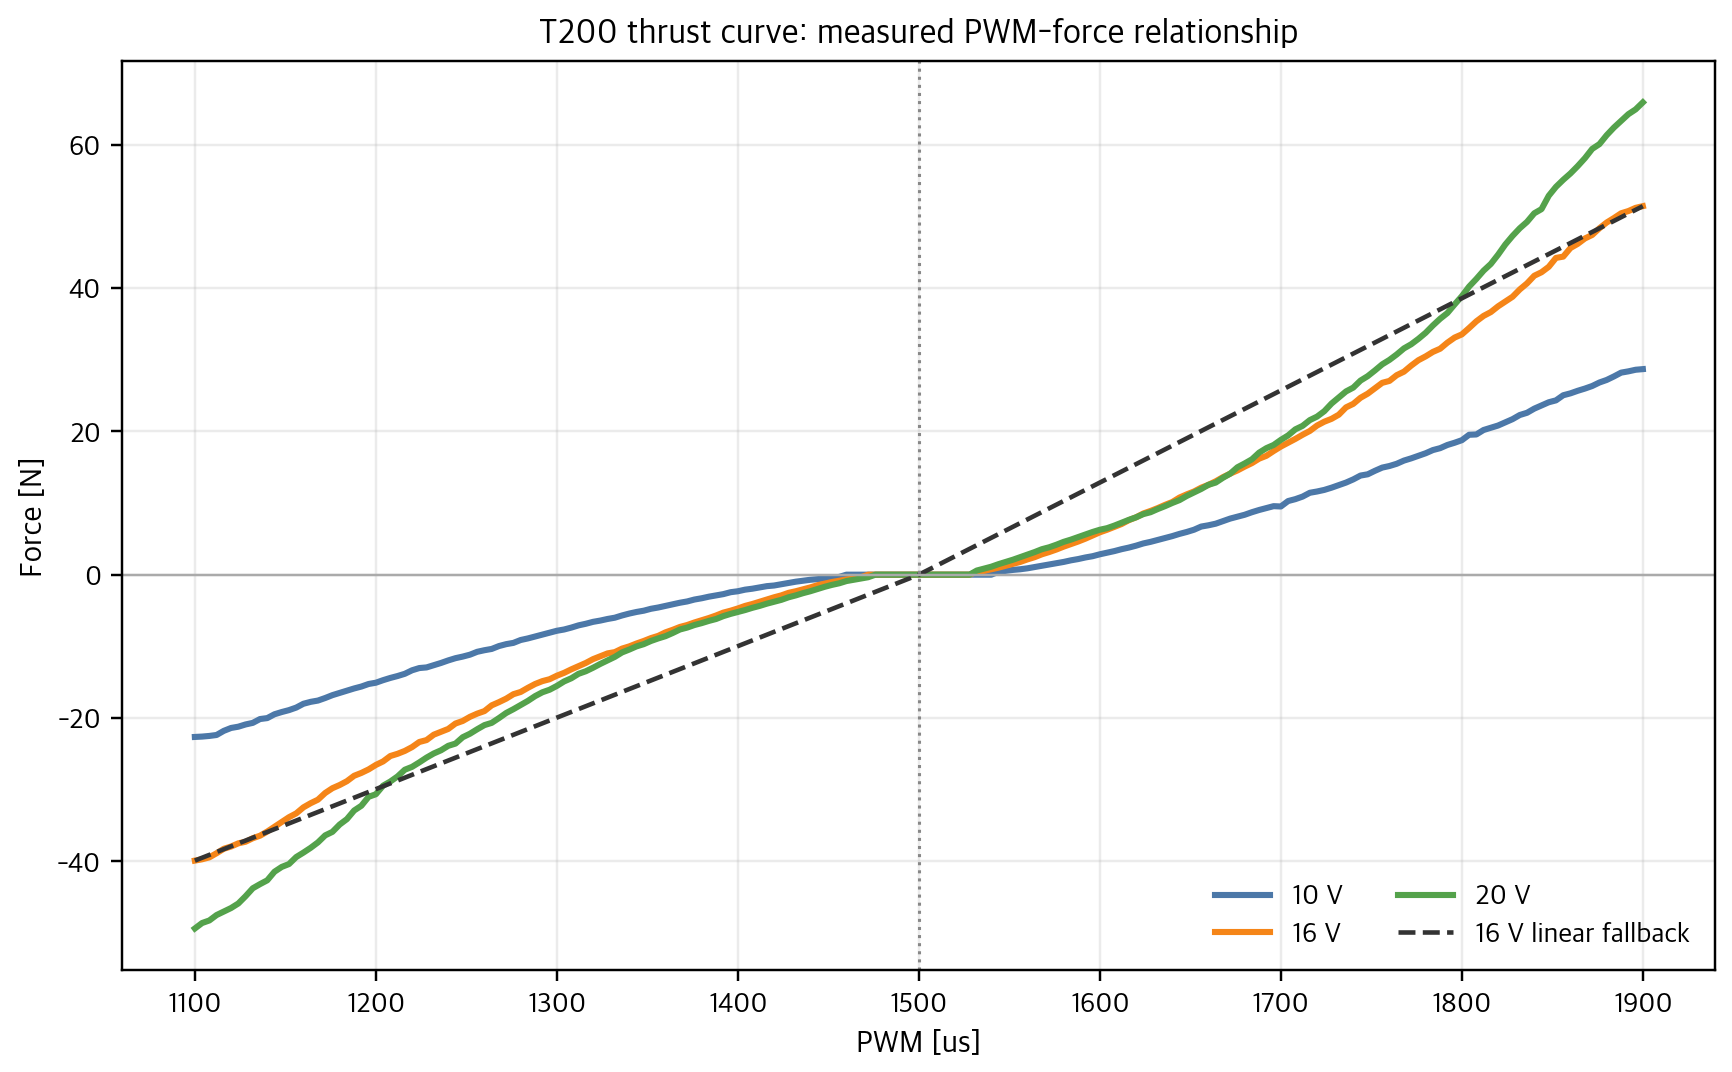
\includegraphics[width=0.92\linewidth]{figures/thruster_curve_comparison.png}
  \caption{T200 공개 성능 데이터 기반 PWM-force 곡선. 10V, 16V, 20V 곡선을 함께 그렸고, 16V에서 단순 선형 fallback을 점선으로 비교했다. 이 그래프는 ``왜 thrust를 선형으로 두지 않았는가''를 가장 직접적으로 보여준다. 실제 추력은 PWM에 대해 비선형이며, 전압에 따라 전체 force envelope도 달라진다.}
\end{figure}

이 그림의 의미는 다음과 같다.

\begin{itemize}[leftmargin=2em]
  \item 같은 PWM 증가가 항상 같은 force 증가를 만들지 않는다.
  \item 전압이 낮아지면 같은 PWM에서도 사용할 수 있는 최대 thrust가 작아진다.
  \item 따라서 sim2real gap을 줄이려면 thrust를 단순 선형 actuator로 놓는 것보다, 실제 공개 곡선을 쓰는 것이 유리하다.
\end{itemize}

\subsection{현재 \texttt{custom} hydrodynamic 계수}

\begin{figure}[htbp]
  \centering
  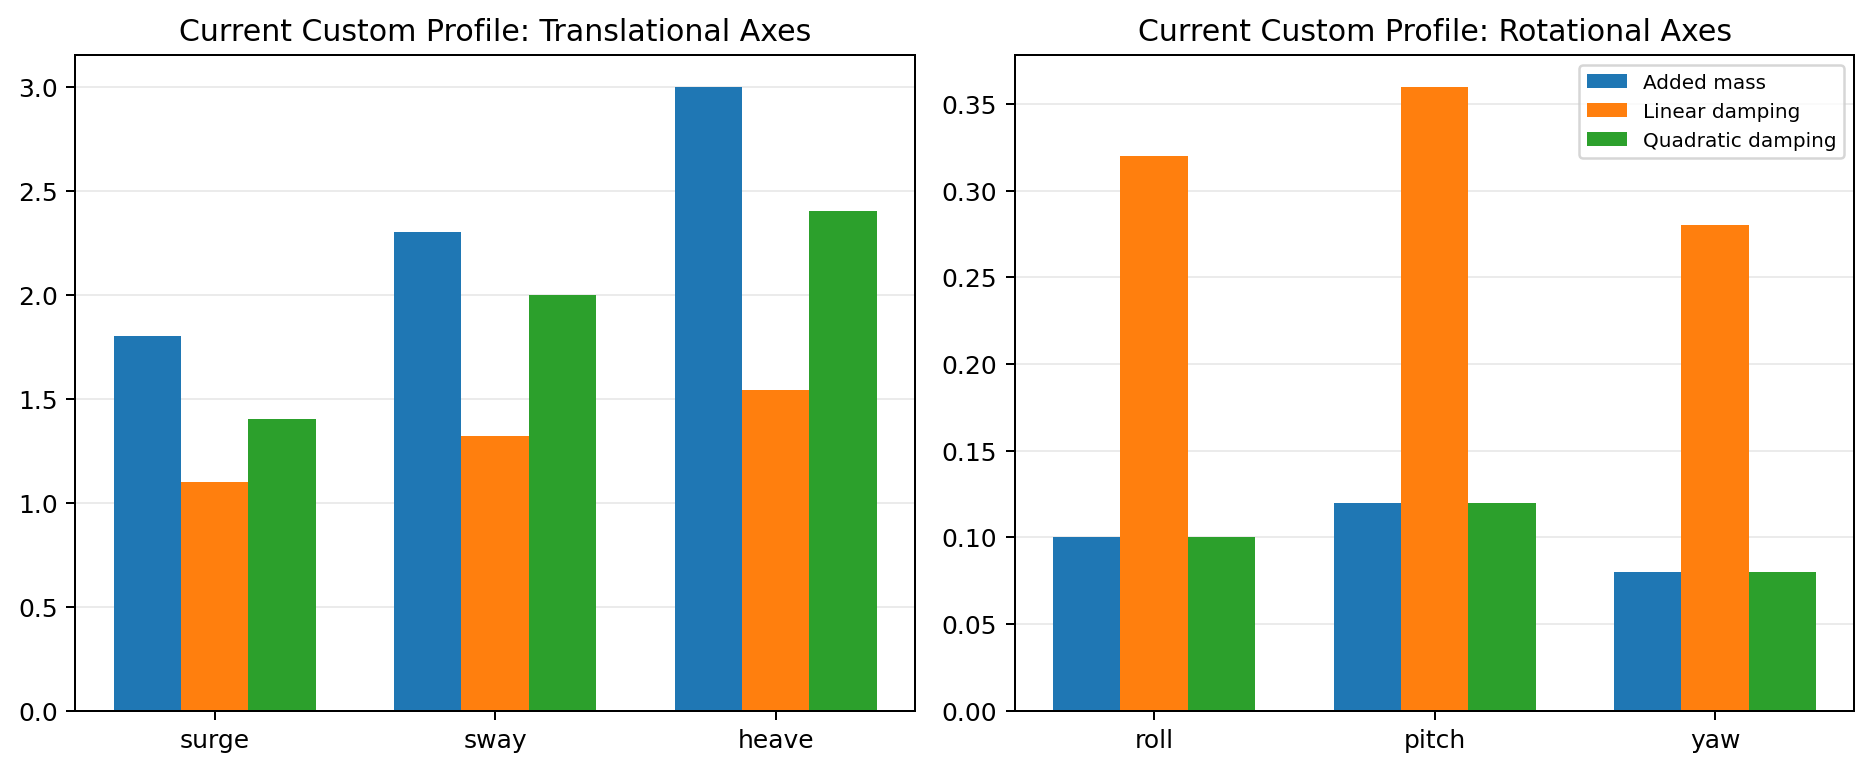
\includegraphics[width=0.96\linewidth]{figures/active_custom_hydrodynamic_coeffs.png}
  \caption{현재 active \texttt{custom} profile에서 사용되는 hydrodynamic coefficients. 병진 축과 회전 축에 대해 added mass, linear damping, quadratic damping을 함께 나타냈다. 이 그림은 현재 active runtime의 coefficient-based 6-DOF 설정을 직접 시각화한 것이다.}
\end{figure}

이 그래프에서 볼 수 있는 핵심은 다음과 같다.

\begin{itemize}[leftmargin=2em]
  \item 축별로 계수가 다르다. 즉 surge, sway, heave가 동일하게 취급되지 않는다.
  \item 회전 축 damping은 자세 안정화와 yaw 응답을 고려해 별도 조정됐다.
  \item added mass와 damping을 동시에 사용해야 실제 수중체의 ``무겁고 감쇠된'' 느낌이 나온다.
\end{itemize}

\subsection{현재 모델의 잠김비-부력 곡선}

\begin{figure}[htbp]
  \centering
  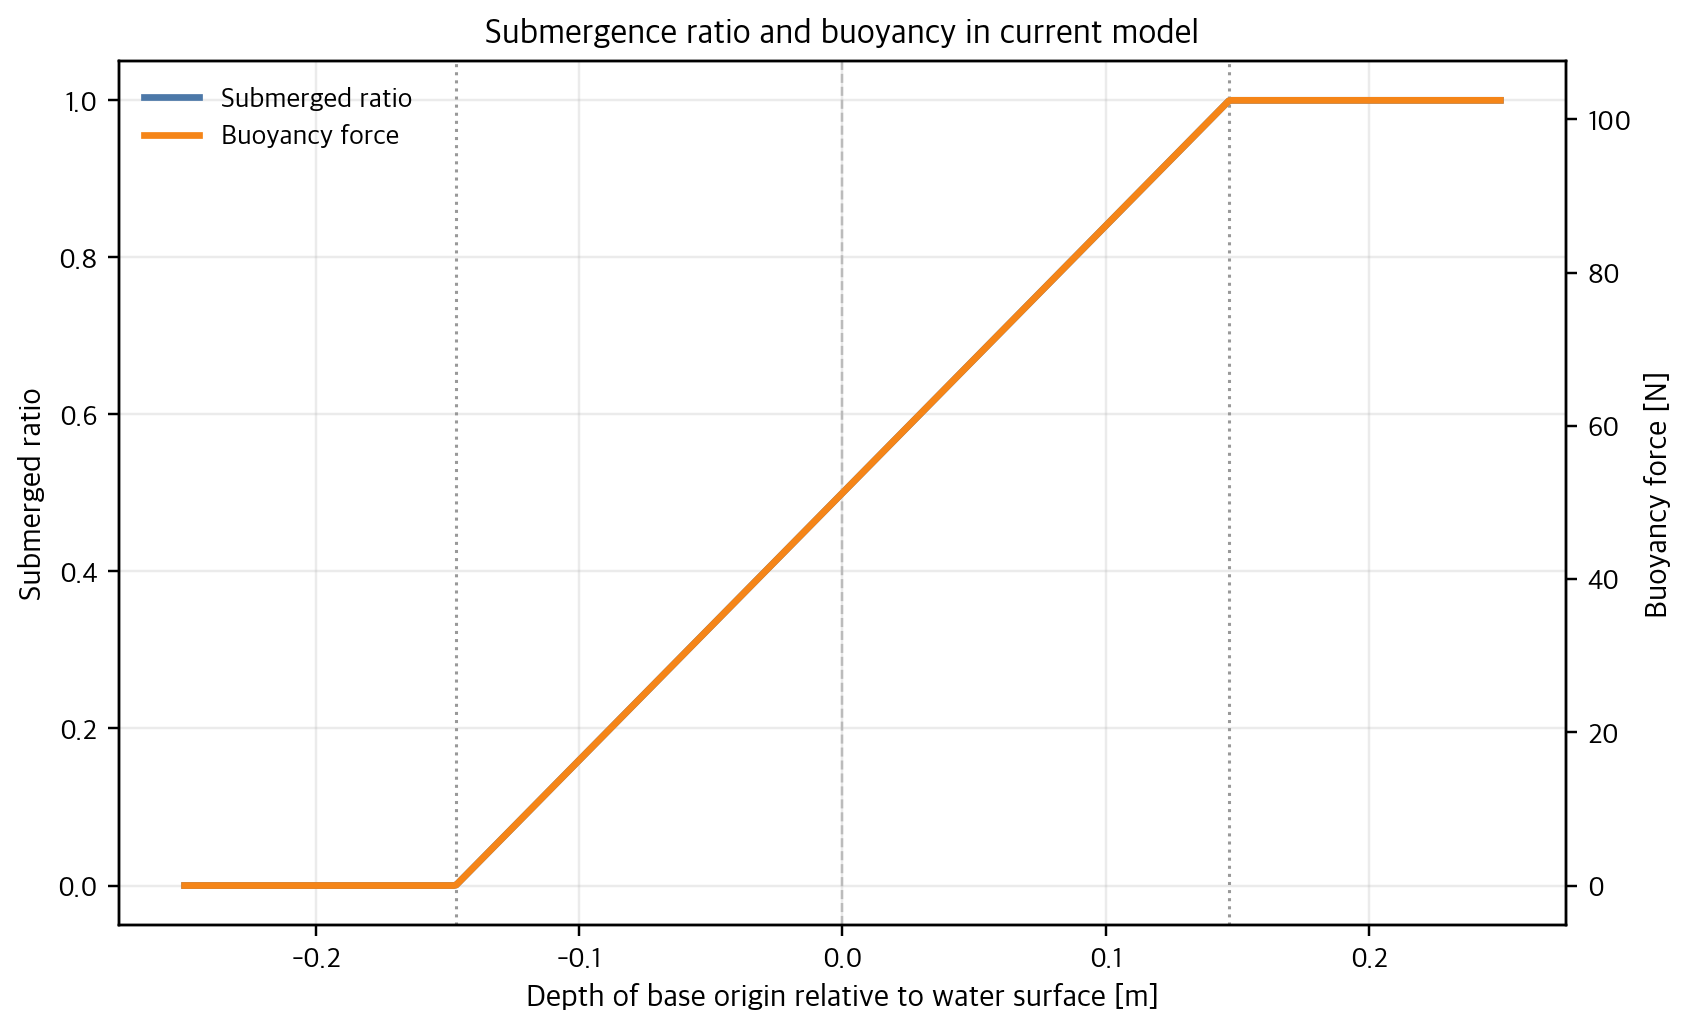
\includegraphics[width=0.92\linewidth]{figures/buoyancy_submergence_curve.png}
  \caption{현재 모델의 잠김비와 부력 곡선. depth가 증가하면 submerged ratio가 선형으로 증가하고, 그에 따라 buoyancy가 최대값까지 선형적으로 올라간다. 이는 현재 코드가 사용하는 단순화된 hydrostatic approximation을 시각적으로 보여준다.}
\end{figure}

이 그림은 현재 buoyancy model의 단순화 수준을 잘 보여준다.

\begin{itemize}[leftmargin=2em]
  \item 완전히 잠기기 전까지는 부력이 선형적으로 증가한다.
  \item 이는 exact submerged-volume 계산이 아니라, 현재 구현의 계산 효율과 단순성을 우선한 근사 모델이다.
  \item 발표 때 ``왜 부력을 복잡한 volume intersection 대신 이렇게 처리했는가''를 설명할 때 유용하다.
\end{itemize}

\section{현재 프로젝트를 설명할 때의 정확한 표현}

현재 구현을 발표나 문서에서 설명할 때는 다음처럼 말하는 것이 가장 정확하다.

\begin{quote}
현재 active simulator는 두 경로를 가진다. 기본 \code{custom} 경로는 MuJoCo를 강체 적분 엔진으로 사용하고 그 위에 custom 6-DOF underwater hydrodynamics를 외력 형태로 얹는다. 비교용 \code{ellipsoid} 경로는 MuJoCo built-in ellipsoid fluid를 사용한다. 두 경로 모두 동일한 SITL/ROS2/QGC scaffold에서 실행되며, 이전 실험 파일은 \texttt{delete/} 디렉터리로 분리되어 있다.
\end{quote}

즉 다음 표현은 부정확하다.

\begin{itemize}[leftmargin=2em]
  \item ``항상 custom hydrodynamics만 사용한다.''
  \item ``항상 MuJoCo의 ellipsoid fluid model만 사용한다.''
\end{itemize}

반면 다음 표현은 정확하다.

\begin{itemize}[leftmargin=2em]
  \item ``MuJoCo의 rigid-body solver 위에 custom underwater hydrodynamics 경로와 built-in ellipsoid fluid 경로를 함께 유지한다.''
  \item ``custom 경로에서는 shape-based ellipsoid approximation을 이용해 hydrodynamic coefficient baseline을 생성할 수 있다.''
\end{itemize}

\section{향후 개선 방향}

향후 방향은 크게 두 가지다.

\subsection{방향 1: 현재 custom model 유지 + 보정 강화}

이 방향은 현재 구조를 유지하면서 다음을 강화하는 것이다.

\begin{itemize}[leftmargin=2em]
  \item 실측 로그 기반 coefficient identification
  \item current / turbulence / wave disturbance 모델 확장
  \item thruster lag / deadzone / asymmetry 보정
\end{itemize}

장점은 현재 control stack과 연동하기 쉽고, 계수 조정이 직관적이라는 점이다.

\subsection{방향 2: MuJoCo built-in ellipsoid model과 비교 실험}

이 방향은 scene에 실제로 \texttt{fluidshape="ellipsoid"} 와 \texttt{fluidcoef} 를 넣어 MuJoCo 공식 fluid model을 활성화하고, 현재 custom model과 비교하는 것이다.

이 경우 비교 대상은 다음이 된다.

\begin{itemize}[leftmargin=2em]
  \item MuJoCo 공식 passive ellipsoid fluid model
  \item 현재 repository의 custom 6-DOF hydrodynamics
\end{itemize}

이를 통해 다음 질문에 답할 수 있다.

\begin{itemize}[leftmargin=2em]
  \item MuJoCo built-in model만으로도 충분한가?
  \item added mass / lift / damping 표현에서 어느 쪽이 더 현실적인가?
  \item real-time 성능 대비 정확도는 어느 쪽이 유리한가?
\end{itemize}

\section{결론}

MuJoCo 공식 문서의 fluid-force 모델은 매우 유용한 출발점이며, 특히 ellipsoid-based model은 added mass, drag, Magnus lift, Kutta lift까지 포함하는 풍부한 현상론적 모델이다.

현재 UUV 프로젝트의 중요한 점은 ``MuJoCo를 썼다''가 아니라, \textbf{동일한 simulator scaffold 위에서 custom hydrodynamics 경로와 built-in ellipsoid 경로를 실제로 비교 가능한 형태로 운영하고 있다는 점}이다.

이번 문서에서 새로 추가한 정량 비교 결과는 다음을 보여준다.

\begin{itemize}[leftmargin=2em]
  \item \textbf{Current Custom} 은 현재 active thrust / actuator 설정 때문에 archived legacy보다 매우 공격적이며, 전진과 yaw authority는 크게 늘었지만 pitch coupling도 크게 증가했다.
  \item \textbf{Current Ellipsoid} 는 peak surge와 peak yaw rate는 custom보다 작지만, peak pitch와 residual yaw를 크게 줄여 \textbf{보다 안정적인 조이스틱 추종 baseline}을 제공한다.
  \item 따라서 현재 코드 상태에서 ``차이를 가장 명확히 보여주는 특별한 부분''은 \textbf{Current Ellipsoid가 legacy 수준의 pitch disturbance를 유지하면서도 active runtime 수준의 actuator authority를 상당 부분 확보한다}는 점이다.
\end{itemize}

따라서 현재 프로젝트의 가장 정확한 요약은 다음과 같다.

\begin{quote}
MuJoCo를 강체 적분 엔진으로 사용하고, \code{custom} 과 \code{ellipsoid} 두 active runtime 경로를 유지하는 underwater simulation stack이다. 기본 경로에서는 coefficient-based 6-DOF hydrodynamics를 직접 계산하고, 비교 경로에서는 MuJoCo built-in ellipsoid fluid를 사용한다. 또한 archived legacy 경로까지 복원해 세 경로의 forward / yaw 응답 차이를 정량 그래프로 비교할 수 있다.
\end{quote}

\section*{참고 문헌}

\begin{itemize}[leftmargin=2em]
  \item MuJoCo Read the Docs, Fluid forces.\\
  \url{https://mujoco.readthedocs.io/en/stable/computation/fluid.html}
  \item MuJoCo XML Reference, \texttt{geom/fluidshape}, \texttt{geom/fluidcoef}.\\
  \url{https://mujoco.readthedocs.io/en/3.2.6/XMLreference.html}
\end{itemize}

\end{document}
